%-----------------------------------------------------------------------------
%
%               Template for sigplanconf LaTeX Class
%
% Name:         sigplanconf-template.tex
%
% Purpose:      A template for sigplanconf.cls, which is a LaTeX 2e class
%               file for SIGPLAN conference proceedings.
%
% Guide:        Refer to "Author's Guide to the ACM SIGPLAN Class,"
%               sigplanconf-guide.pdf
%
% Author:       Paul C. Anagnostopoulos
%               Windfall Software
%               978 371-2316
%               paul@windfall.com
%
% Created:      15 February 2005
%
%-----------------------------------------------------------------------------


\documentclass[preprint]{sigplanconf}

% The following \documentclass options may be useful:

% preprint      Remove this option only once the paper is in final form.
% 10pt          To set in 10-point type instead of 9-point.
% 11pt          To set in 11-point type instead of 9-point.
% authoryear    To obtain author/year citation style instead of numeric.

\usepackage{azalea}


\begin{document}

\special{papersize=8.5in,11in}
\setlength{\pdfpageheight}{\paperheight}
\setlength{\pdfpagewidth}{\paperwidth}

\conferenceinfo{CONF 'yy}{Month d--d, 20yy, City, ST, Country} 
\copyrightyear{20yy} 
\copyrightdata{978-1-nnnn-nnnn-n/yy/mm} 
\doi{nnnnnnn.nnnnnnn}

% Uncomment one of the following two, if you are not going for the 
% traditional copyright transfer agreement.

%\exclusivelicense                % ACM gets exclusive license to publish, 
                                  % you retain copyright

%\permissiontopublish             % ACM gets nonexclusive license to publish
                                  % (paid open-access papers, 
                                  % short abstracts)

%\titlebanner{banner above paper title}        % These are ignored unless
%\preprintfooter{short description of paper}   % 'preprint' option specified.

\title{CoLoSL: Concurrent Local Subjective Logic}
\subtitle{}

%% \authorinfo{Azalea Raad\and Jules Villard \and Philippa Gardner}
%%            {Imperial College London}
%%            {\{azalea, j.villard, pg\}@@imperial.ac.uk}
\authorinfo\null\null\null

\maketitle

\begin{abstract}
A key difficulty in verifying shared-memory concurrent programs is
reasoning compositionally about each thread in isolation. Existing
verification techniques for fine-grained concurrency require global
reasoning about shared resource, impeding compositionality.  This
paper introduces the program logic CoLoSL, in which each thread is
verified with respect to its subjective view of the shared state,
tailored down to only those shared resources accessed by the
thread. Subjective views may arbitrarily overlap with each other.
This flexibility provides truly compositional proofs for shared-memory
concurrency, which we demonstrate on a range of examples including a
concurrent computation of the spanning tree of a graph.
\end{abstract}


\category{\hspace*{-.8em}F.3.1}{Specifying and Verifying and Reasoning about
  Programs}{Logics of programs}%, Specification techniques}
\category{D.2.4}{Software/Program Verification}{Correctness proofs, Formal methods}

% general terms are not compulsory anymore, 
% you may leave them out
%% \terms
%% term1, term2

\keywords
Concurrency, Program logic, Compositional reasoning, Separation logic

\section{Introduction}

%% Jules: be more general than just program logics? Model-checking,
%% etc.?


%\pg{This is what we should answer by the introduction: 
%What's the problem with the current state of the art?
%What is our solution?
%Why is the problem we're solving hard?
%How do we solve the challenges?
%Why do we do better than existing work?
%What are the lessons learnt from the paper?}


A key difficulty in verifying properties of shared-memory concurrent
programs is to be able to reason compositionally about each thread in
isolation, even though in reality the correctness of the whole system
is the collaborative result of intricately intertwined actions of the
threads.  Such compositional reasoning is essential for verifying
large concurrent systems, library code and more generally incomplete
programs, and for replicating a programmer's intuition about why their
implementations are correct.

Separation logic reasoning~\cite{seplog,csl-tcs} has
been used to demonstrate the importance of reasoning about only the
portions of the local machine state (the resource) actually accessed
by programs. Recently, several techniques have been built on top of
separation logic, such as those related to CAP
reasoning~\cite{cap-ecoop10,icap,tada}, which have made substantial advances in
fine-grained compositional reasoning about complex algorithms which
access the global shared state.  However, the rigidity of existing
techniques forces us to work with {\em static} global shared state,
such as a shared data structure for representing sets, even though a
thread might only access just a small part of it.  This global state
must be robust with respect to all possible interferences from the
environment, {even on parts of the shared state not actually accessed
  by the current thread}. Intuitively, compositionality calls for
reasoning that only refers to the part of the global shared state actually
accessed by each thread.  Existing reasoning techniques are too rigid
to achieve this. 



This paper introduces the program logic \colosl, where  threads access one
global shared state and are verified with respect to their
\emph{subjective views} of this state. Each
subjective (personalised) view  is an assertion which provides a thread-specific description
of part of the shared state. It describes 
the partial shared resource necessary
for the thread to run and the  thread-specific interference 
describing how the thread and the environment can effect this partial
shared resource. Subjective views may arbitrarily overlap with each
other, and subtly expand and contract to the natural resources and the 
interference required by  the current thread. 
This flexibility
provides truly compositional reasoning  for shared-memory concurrency.


%This paper presents the program logic \colosl, which achieves
%compositional reasoning for concurrent programs by enabling
%\emph{subjective} views of the shared state. Subjective views may be
%composed arbitrarily and manipulated so as to retain only the portions
%of local and shared state actually accessed by each thread in the
%program, and to consider only the interferences relevant to that piece
%of shared state. \colosl achieves a greater degree of compositionality
%than existing work by enabling \emph{finer-grained} sharing: the
%program logic can consider that threads share only what is relevant to
%their function, a key ingredient of compositionality.



%Driven by the ever-increasing need for concurrency in software,
%%  spurred by recent hardware developments, 
%program logics for shared-memory concurrency have progressed towards
%the twin ideals of fine-grain reasoning and compositionality. The
%former enables elegant proof techniques about increasingly subtle
%concurrency idioms~\cite{vv06popl,vv07msc,todo}, while the latter
%allows programs to be proved component-wise and their proofs to be
%reusable as-is in any client
%program~\cite{csl-tcs,cap-ecoop10,icap}.
%%  Central to these compositional verification frameworks is the
%% formalism used to describe both the state shared between program
%% threads and the possible interference on that state.
%%
%% dating back from Owicki~\cite{owicki}, and later Jones who
%% integrated the notion of interference in the logic
%% itself~\cite{rg}.
%% 

%% Consider for instance
%% a program where threads operate on subgraphs of a global graph.


%%  dubbed their \emph{subjective states}.  One may then reuse these
%%   specifications in the context of any larger local state (as is
%%   standard in separation logic~\cite{rey02}), and, crucially for
%%   compositional reasoning about concurrent programs, any larger
%%   shared state. The subjective states of different threads in a
%%   program are allowed to overlap arbitrarily, ensuring maximum
%%   reusability of proofs.


%\colosl assertions comprise standard assertions from the
%separation-logic literature~\cite{rey02,ramification}, plus {\em
%  subjective views} and {\em capabilities}. 

A subjective view
$\shared{P} I$ comprises an  assertion $P$ which gives {\em partial}
information about the global shared state and interference assertion
$I$ which describes how this partial shared state may be changed by
the thread or the environment. The interference assertion $I$ declares
actions of the form $\token a : P' \swap Q$, with capability assertion
$[\token a]$ providing a thread with permission to use this action
$\token a$. Subjective views expand or contract depending on the resource required
by the thread, which has subtle consequences for the logical
reasoning. In particular, it is possible to strengthen actions in $I$
to record  some global information known to the subjective view.
Then, the view can be weakened to just 
the resources and possibly strengthened
actions appropriate to  the thread. The strengthened actions retain  some
global information despite the weakened view. 


We introduce several novel reasoning principles which allow us to expand and
contract subjective views. Subjective views can always be duplicated
using the \copyRule  principle:
\begin{align*}
  \label{eq:split}
  \shared{P}{I} &=> \shared{P}{I} * \shared P I \tag{\copyRule}
\end{align*}
In combination with the usual law of parallel composition of
separation logic~\cite{csl-tcs}, this yields a powerful mechanism to
distribute the shared state between several threads:
\[
\infer[\parRule]
        {\hoare{P_1 * P_2}{\mathbb{P}_1 || \mathbb{P}_2}{Q_1 * Q_2}}
        {\hoare{P_1}{\mathbb{P}_1}{Q_1} &
          \hoare{P_2}{\mathbb{P}_2}{Q_2}}
\]
The subjective views of each thread will be typically
too strong, describing resource that is not necessary being used by
the thread. However, before  weakening the view, it will sometimes 
be useful to strengthen some of the actions in the interference assertion
to preserve global knowledge. We achieve this using the \shiftRule~principle:
\begin{align*}
  \label{eq:shift}
  I \weakenIb{P} I'
  &\text{ implies }
  \shared{P}{I} ===> \shared{P}{I'}
  \tag{\shiftRule}
\end{align*}
This principle states that an interference assertion $I$ can be
exchanged for any other interference assertion $I'$ that has the same projected
effect on the subjective state $P$. When this is the case, we write $
I \weakenIb{P} I'$ and say that the actions have been  \emph{shifted}. It can
be used to strengthen actions given by the combined global knowledge
arising form the combination of $I$ and $P$. It can also be used to forget actions
which are not relevant to $P$. This \shiftRule 
principle describes a flexible  behaviour of interference  which is 
in marked  contrast with most existing formalisms, where 
interference is fixed throughout the verification of the whole
program.


Now, with a possibly strengthened interference assertion, we are able 
to use the 
 \forgetRule principle to zoom  on the resource required by the current thread:
\begin{align*}
  \label{eq:forget}
  \shared{P * Q}{I} &=> \shared{P}{I}  \tag{\forgetRule}
\end{align*}
We  can again use the \shiftRule  principle to, this time, forget some of
the actions not now relevant to the subjective view. Finally, as usual, we must
{\em stabilise} the assertion of the subjective view,  so that the view is
robust with respect to interferences from the environment. If the
knowledge given by the 
combination of the assertion $P$ and the interference assertion $I$ is too weak, then this stabilisation results in
a precondition that is too weak. 


These reasoning principles enable us to provide subjective views for
the threads which are just right. 
We can proceed to verify the threads, knowing that their
subjective views describe personalised preconditions which only  
describe the resource relevant to the individual threads. The
resulting postconditions naturally describe
overlapping parts of the shared state, which are then joined together
using the disjoint concurrency rule and the \mergeRule principle:
\begin{align*}
  \label{eq:merge}
  \shared{P}{I_1} * \shared{Q}{I_2} &=> \shared{P \sepish Q}{I_1 \cup I_2} \tag{\mergeRule}
\end{align*}
The assertion $P ** Q$ 
describes the overlapping of states arising from $P$ and $Q$, using
the overlapping conjunction $**$~\cite{ramification,js-popl12}. 
The new
interference relation is simply the union of previous
interferences. Finally, we can use the \shiftRule principle to simplify the
interference assertion now that we are back with a larger subjective view.

The last principle to mention is how subjective views are created
using the \extendRule principle, where $\vec a, \vec b$ range over
tokens:

\begin{align}
  \label{eq:extend}
  P \containI I
  &\text{ implies }
  P ===>
  \exsts{\vec{{a}}, \vec{{b}}}[{a}_1] {*} \cdots {*}
        [ a_n] * \shared{P *
   [{b}_1] {*} \cdots {*} [{b}_n]}{I}
  \tag{\extendRule}
\end{align}
%
The side condition $P \containI I$ ensures that the actions associated
with interference assertion $I$ are confined to $P$. The existential
quantification of tokens is to ensure the \emph{freshness} of
the generated capabilities. 
The main novelty of this rule is the fact
that new actions may refer to existing shared state, as we shall see  in
our set example discussed below. Notice that we  do not require a corresponding principle for destroying
subjective views since this is achieved by the \forgetRule principle. 


With these reasoning principles, we are able to expand and contract
subjective views  to provide just the resource required by a thread.
In essence, we provide  frame-like reasoning for  subjective  views. 
%% The interaction between  these principles is
%% subtle. We are able to forget resource of the subjective assertion $P$
%%  whilst at the same time adapting the interference relation $I$  to
%% capture global constraints associated with that lost resource.
In 
\S\ref{sec:intuition}, we 
demonstrate this using 
a variant of the famous  token ring mutual exclusion algorithm~\cite{dijkstra74},
introduced by Dijkstra to illustrate distributed, global knowledge between
threads. The point is that, as well as local knowledge
about how the threads behave, the programmer also has global knowledge
about how the threads constrain each other. Our reasoning captures the
spirit of reasoning locally about individual threads at the same time
as retaining global knowledge about the overall thread behaviour. It
is a good  introductory example, as it uses all the highlighted \colosl
reasoning principles in a fundamental way. 

In \S\ref{sec:logic}, we interpret \colosl assertions
 over a particular domain which includes: thread-local
state exclusively visible to the thread; {\em one} global shared state
accessible by all thread (in contrast with the CAP approach); and {\em
  action models} describing how the global state can be updated.  In
\S\ref{sec:semantics}, we define the rely and guarantee conditions
of each thread is in terms of their action models, and provide a
sketch of soundness. In particular, the
reasoning principles highlighted above are simple semantic
consequences of our generic model of program states.  The full
technical details can
be found 
in the accompanying technical report~\cite{colosl-tr14}.



In \S\ref{sec:examples}, we study two further, more challenging
examples. We verify a concurrent spanning tree algorithm for
graphs. This algorithm uses threads spawned on arbitrary overlapping
graphs. We demonstrate that the flexible, overlapping subjective views
of \colosl are just what we need.  We also verify a concurrent set
module implemented using a hand-over-hand list-locking algorithm.
%Interestingly, this
%example uses the \extendRule principle   to the create new actions which refer to existing
%state in a fundamental way. 
The flexibility of \colosl's subjective views  leads to a
considerably simpler correctness proof compared to that of CAP. 



\section{Informal development}
\label{sec:intuition}

Let us showcase all four new reasoning principles of \colosl by
sketching a proof of a simple, if slightly artificial example (we will
turn our attention to less contrived examples in
\S\ref{sec:examples}).

Consider the program $\mathbb{P}$ of \fig\ref{fig:concurrentInc},
written in pseudo-code, where variables $x$, $y$ and $z$ are allocated
on the heap and variable reading and mutation are understood as the
corresponding heap operations. After initialisation of the variables
to $0$, three threads are spawned to increment their values in
lock-step: $\mathbb{P}_x$ is the first allowed to run its increment
operation, then $\mathbb{P}_y$ and finally $\mathbb{P}_z$. This
process repeats until $x = y = z = 10$.

\begin{figure*}
\centering
\begin{tabular}{@{}l@{\ }|@{\ }l@{\ }|@{\ }l@{\ }|@{\ }l@{}}
  {$\mathbb{P}_x$:}& 
  {$\mathbb{P}_y$:}& 
  {$\mathbb{P}_z$:}&
  $\mathbb{P}$:\\[.5ex]
\begin{lstlisting}
//$\comment\{\shared{\cell{x}{0} * \cell{z}{0}}{I_x} * \token a_x\}$
while($x$ != 10)
//$\comment\left\{\shared{\begin{array}{@{}l<{\null}@{}l<{\null}@{}}\exsts{v}\cell{x}{v} * \cell{z}{v} \lor\\ \cell{x}{v+1} * \cell{z}{v}\end{array}}{I_x}\!\!\!\!\!\! * \token a_x\right\}$
{ $\langle$if ($x$ == $z$) $x$++;$\rangle$ }
//$\comment\left\{\shared{\begin{array}{@{}l<{\null}@{}l<{\null}@{}}\cell{x}{10} * \cell{z}{10} \lor\\ \cell{x}{10} * \cell{z}{9}\end{array}}{I_x}\!\!\!\!\!\! * \token a_x\right\}$
\end{lstlisting}
&
\begin{lstlisting}
//$\comment\left\{\shared{\begin{array}{@{}l<{\null}@{}l<{\null}@{}}\cell{x}{0} * \cell{y}{0} \lor\\ \cell{x}{1} * \cell{y}{0}\end{array}}{I_y}\!\!\!\!\!\! * \token a_y\right\}$
while($y$ != 10)
//$\comment\left\{\shared{\begin{array}{@{}l<{\null}@{}l<{\null}@{}}\exsts{v}\cell{x}{v} * \cell{y}{v} \lor\\ \cell{x}{v+1} * \cell{y}{v}\end{array}}{I_y}\!\!\!\!\!\! * \token a_y\right\}$
{ $\langle$if ($y$ < $x$) $y$++;$\rangle$ }
//$\comment\left\{\shared{\begin{array}{@{}l<{\null}@{}l<{\null}@{}}\cell{x}{10} * \cell{y}{10} \lor\\ \cell{x}{11} * \cell{y}{10}\end{array}}{I_y}\!\!\!\!\!\! * \token a_y\right\}$
\end{lstlisting}
&
\begin{lstlisting}
//$\comment\left\{\shared{\begin{array}{@{}l<{\null}@{}l<{\null}@{}}\cell{y}{0} * \cell{z}{0} \lor\\ \cell{y}{1} * \cell{z}{0}\end{array}}{I_z}\!\!\!\!\!\! * \token a_z\right\}$
while($y$ != 10)
//$\comment\left\{\shared{\begin{array}{@{}l<{\null}@{}l<{\null}@{}}\exsts{v}\cell{y}{v} * \cell{z}{v} \lor\\ \cell{y}{v+1} * \cell{z}{v}\end{array}}{I_z}\!\!\!\!\!\! * \token a_z\right\}$
{ $\langle$if ($z$ < $y$) $z$++;$\rangle$ }
//$\comment\left\{\shared{\begin{array}{@{}l<{\null}@{}l<{\null}@{}}\cell{y}{10} * \cell{z}{10} \lor\\ \cell{y}{11} * \cell{z}{10}\end{array}}{I_z}\!\!\!\!\!\! * \token a_z\right\}$
\end{lstlisting}
&
\begin{lstlisting}
//$\comment\{x|-> - * y|-> - * z|-> - \}$
$x$ = 0; $y$ = 0; $z$ = 0;
//$\comment\{x|-> 0 * y|-> 0 * z|-> 0 \}$
//$\comment\left\{\begin{array}{@{}l<{\null}@{}l<{\null}@{}}\shared{x|-> 0 * y|-> 0 * z|-> 0} I\\ \null*\token a_x * \token a_y * \token a_z\end{array}\right\}$
($\mathbb{P}_x$ || $\mathbb{P}_y$ || $\mathbb{P}_z$)
//$\comment\left\{\begin{array}{@{}l<{\null}@{}l<{\null}@{}}\shared{x|-> 10 * y|-> 10 * z|-> 10} I\\ \null*\token a_x * \token a_y * \token a_z\end{array}\right\}$
\end{lstlisting}
\end{tabular}

\begin{align*}
  I_x &\eqdef \left\{
  \begin{array}{@{}l@{}}
    \token a_x:\, \exsts{v} \cell{x}{v} * \cell{z}{v}  \swap  \cell{x}{v+1} * \cell{z}{v}\\
    \token a_z:\, \exsts{v} \cell{x}{v+1} * \cell{y}{v+1} * \cell{z}{v}\swap \cell{x}{v+1} * \cell{y}{v+1} * \cell{z}{v+1}
  \end{array}
  \right.\\
  I_y &\eqdef \left\{
  \begin{array}{@{}l@{}}
    \token a_x:\, \exsts{v} \cell{x}{v} * \cell{y}{v} * \cell{z}{v}  \swap  \cell{x}{v+1} * \cell{y}{v} * \cell{z}{v}\\
    \token a_y:\, \exsts{v} \cell{x}{v+1} *  \cell{y}{v}\swap \cell{x}{v+1} * \cell{y}{v+1}
  \end{array}
  \right.\\
  I_z &\eqdef \left\{
  \begin{array}{@{}l@{}}
    \token a_y:\, \exsts{v} \cell{x}{v+1} * \cell{y}{v} * \cell{z}{v}  \swap \cell{x}{v+1} * \cell{y}{v+1} * \cell{z}{v}\\
    \token a_z:\, \exsts{v} \cell{y}{v+1} *  \cell{z}{v}\swap \cell{y}{v+1} * \cell{z}{v+1}
  \end{array}
  \right.\\
  I &\eqdef \left\{
  \begin{array}{@{}l@{\,}l@{}r@{\ }c@{\ }l@{}}
    \token a_x: & \exsts{v} & \cell{x}{v} * \cell{z}{v} & \swap & \cell{x}{v+1} * \cell{z}{v}\\
    \token a_y: & \exsts{v} & \cell{x}{v+1} * \cell{y}{v} & \swap & \cell{x}{v+1} * \cell{y}{v+1}\\
    \token a_z: & \exsts{v} & \cell{y}{v+1} * \cell{z}{v} & \swap & \cell{y}{v+1} * \cell{z}{v+1}
  \end{array}\right.
\end{align*}

\hrule\vspace{5pt}
\caption{The concurrent increment program together with a \colosl proof
  sketch. Lines starting with \lstinline{//} contain formulas that describe
  the local and subjective shared state at relevant program point.}
\label{fig:concurrentInc}
\end{figure*}

\subsection{\colosl assertions}
\label{subsec:intuition}

In this proof sketch, we use \colosl assertions to describe program
states. As will be formalised in \S\ref{sec:logic}, we extend
\emph{separation logic} assertions~\cite{rey02} with subjective views,
and interpret \colosl assertions over a particular domain that
includes a \emph{local} state, a \emph{subjective} state, and
interference \emph{actions}. These instrumented states are linked to
machine states in our soundness proof based on Views and presented in
\S\ref{sec:soundness}. A pointsto predicate $x |-> y$ denotes those
states whose local heap is the singleton heap where the only allocated
address is $x$, and it points to value $y$. An assertion $P_1 * P_2$
splits the local state into two \emph{disjoint} heaps and the
subjective state into two \emph{overlapping} heaps such that the
corresponding substates satisfy $P_1$ and $P_2$, respectively. A
\emph{subjective view} $\shared{P}{I}$ is true if the subjective state
satisfies $P$ and is subject to interferences in $I$.

\begin{figure}
\centering
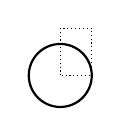
\begin{tikzpicture}
\draw[thick] (0,0) circle (.4cm);
\draw[densely dotted] (0,0) rectangle (.4cm,.6cm);
\end{tikzpicture}
\quad$\swap$\quad
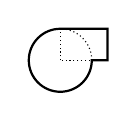
\begin{tikzpicture}
\draw[densely dotted] (0,0) circle (.4cm);
\draw[densely dotted] (0,0) rectangle (.6cm,.4cm);
\draw[thick] (.4cm,0) arc (0:-270:.4cm) -- (.6cm,.4cm) -- (.6cm,0) -- cycle;
\end{tikzpicture}\\


\null\hfill

\begin{tikzpicture}[baseline,yshift=.1cm]
\draw[thick] (0,0) circle (.4cm);
\end{tikzpicture}\quad subjective state
\hfill
$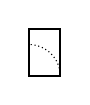
\begin{tikzpicture}[baseline,yshift=-.25cm]
\draw[thick] (0,0) rectangle (.4cm,.6cm);
\draw[densely dotted] (.4cm,0) arc (0:90:.4cm);
\end{tikzpicture}|= P$
\hfill
$
\begin{tikzpicture}[baseline]
\draw[thick,yshift=-.1cm] (0,0) rectangle (.6cm,.4cm);
\end{tikzpicture}|= Q$
\hfill\null

\vspace{5pt}\hrule\vspace{5pt}
\caption{Effect of an action $P\swap Q$.}
\label{fig:action}
\end{figure}

Interferences in $I$ are of the form $\token{a}: P \swap Q$ where
$\token{a}$ denotes a \emph{capability} associated with \emph{action}
$P \swap Q$. $P$ represents the action pre-condition and describes the
part of the shared state required to carry out the action, while $Q$
is the action post-condition and describes the part of the shared
state after the action.  A thread in possession of a given capability
in its local state can perform the associated action and update the
shared state accordingly provided that the contents of the shared
state satisfy the action pre-condition.  For instance, as the name
suggests, the action associated with capability $\token a_x$ in $I_y$,
corresponds to the update of variable $x$: for any $v$, if
$\cell{x}{v} * \cell{y}{v} * \cell{z}{v}$, a thread in possession of
$\token a_x$ in its local state can increment $x$.  A particularity of
\colosl is that actions can be performed by the environment any time
their precondition is \emph{compatible} with the current subjective
state, as represented schematically in \fig\ref{fig:action}, and not
only when the precondition is satisfied by a \emph{substate} of the
subjective state (as is required for the program to perform the
action). In particular, an action whose precondition is satisfiable is
\emph{always} enabled from the empty subjective view (which by
definition is compatible with all other states).

Assertions appearing in pre and postconditions of triples must be
\emph{stable}. That is, for any action permitted by $I$, where $I$ is
the interference relation of a subjective view appearing in the
assertion, if the current thread does not exclusively hold the
associated capability (and thus the action may be performed by the
environment at any time), the assertion must remain true after the
action has taken place (see \fig\ref{fig:action}). For instance, the
assertion
\[
\token a_x * \token a_y * \shared{x|->0 * y|->0}{I_y}
\]
is stable since it owns the capabilities associated with both actions
of $I_y$ ($\token a_x$ and $\token a_y$), hence no other thread can
perform an action that would invalidate $x|->0 * y|->0$. On the other
hand, the assertion
\[
\token a_y * \shared{x|->0 * y|->0}{I_y}
\]
is not stable since a thread in possession of $\token a_x$ can
potentially increment the value of $x$ and thus invalidate $x|->0 *
y|->0$.

%%%%%%%%%%%%%%%%%%%%%%%%%%%%%%%%%%%%%%%%%%
\subsection{Extending the shared region}
\label{subsec:extend}

The program state in \colosl is modelled by two components
representing a thread-local (private) state exclusively visible to the
thread, and a shared state accessible by all threads. At the very
beginning of the execution of $\mathbb{P}$, the state is purely local
and contains the three variables $x$, $y$, and $z$, which allows
$\mathbb P$ to initialise them to 0. Since the purpose of the rest of
the program is to share these variables between $\mathbb P_x$,
$\mathbb P_y$, and $\mathbb P_z$, a shared region is created, ruled by
interferences $I$ and the three tokens $\token a_x$, $\token a_y$, and
$\token a_z$. The capabilities are automatically added to the current
local state upon region creation:
\begin{align}
  \label{eq:extend}
  P \containI I
  &\text{ implies }
  P \Vvdash
  \exsts{\capAss{1}, \capAss{2}} \capAss{1} * \shared{P *
    \capAss{2}}{I}
  \tag{\textsc{Extend}}
\end{align}
A relation $P\Vvdash P'$ means that it is safe to substitute $P$ for
$P'$ (resp.\ $P'$ for $P$) in the precondition (resp.\ postcondition)
of any triple (hence if $P|- P'$ then $P\Vvdash P'$).
\julescomment{TODO: say more about $\Vvdash$, perhaps a reference?}
The existential quantification of capabilities is to ensure the
\emph{freshness} of the generated capabilities. The side condition $P
\containI I$ ensures that the mutations performed by actions in $I$
are confined to $P$, hence do not contradict existing views of the
shared state. This notion will be formalised in
\S\ref{subsec:extension}.


%%%%%%%%%%%%%%%%%%%%%%%%%%%%%%%%%%%%%%%%%
\subsection{Combining Subjective Views}
\label{subsec:merge}

The next step is to distribute the state to the three threads. This is
done, as is standard in variants of separation logic, using the
following concurrency rule:
\[
\infrule{Parallel}
        {\hoare{P_1}{\mathbb{P}_1}{Q_1}\\
          \hoare{P_2}{\mathbb{P}_2}{Q_2}}
        {\hoare{P_1 * P_2}{\mathbb{P}_1 || \mathbb{P}_2}{Q_1 * Q_2}}
        {}
\]



The capabilities $\token a_x$, $\token a_y$ and $\token a_z$ are
passed to $\mathbb P_x$, $\mathbb P_y$ and $\mathbb P_z$. The
subjective shared state is split using $*$ and the following principle
of \colosl:
\begin{align*}
  \shared{P}{I_1} * \shared{Q}{I_2} &\vdash \shared{P \sepish Q}{I_1 \cup I_2} \tag{\textsc{Merge}}
\end{align*}
Since a shared state assertion $\shared{P}{I}$ defines contents of
parts of the shared state, multiple threads can view different,
potentially overlapping parts of the shared state. As such, the
separating conjunction $*$ behaves as \emph{overlapping conjunction}
$\sepish$~\cite{rey-slnotes,ramification} (sometimes called
\emph{sepish}~\cite{gareth-js12}).

Consequently, as in the case of the first and second lines of the
above derivation $\shared{P_0}{I} * \shared{P_0}{I} \iff
\shared{P_0}{I}$. Upon dividing the capabilities between the three
threads, the $\shared{P_0}{I}$ assertion is no longer stable and is
thus weakened into the stable assertion $G$. Predicate $G$ describes
the contents of the shared state as three disjuncts corresponding to
various points in execution of $\mathbb{P}$.


In order to establish the desired post-condition, at this stage we
need to \emph{merge} the subjective views of all three threads and
obtain a stronger view such as that of $G'$ in
\fig\ref{fig:concurrentIncCoLoSLSpec}.
\begin{align*}
  \label{eq:merge}
  \shared{P}{I_1} * \shared{Q}{I_2} &\vdash \shared{P \sepish Q}{I_1 \cup I_2} \tag{\textsc{Merge}}
\end{align*}
By two applications of the \textsc{Merge} rule, we can merge $S'_x$,
$S'_y$ and $S'_z$ and obtain $\shared{\cell{x}{10} * \cell{y}{10} *
  \cell{z}{10}}{I_x \cup I_y \cup I_z}$. Finally, through an
application of \textsc{Shift} rule, we can rewrite $I_x \cup I_y \cup
I_z$ into $I$ as specified in \fig\ref{fig:concurrentIncCoLoSLSpec}
and obtain $G'$.



%%%%%%%%%%%%%%%%%%%%%%%%%%%%%%%%%%%%%%
\subsection{Forgetting shared state}
\label{subsec:hide}

We are now left with justifying the proofs of each individual thread,
made in isolation.

Note that thread $\tau_x$ is only concerned with the values of $x$ and
$z$; \emph{mutatis mutandis} for $\tau_y$ and $\tau_z$. However, with
the specification of \fig\ref{fig:concurrentIncCoLoSLSpec}, all three
variables are visible by $\tau_x$ and as such in verification of
$\mathbb{P}_x$ it is necessary to account for the interference
associated with $y$ even though its value is neither read nor modified
by $\tau_x$. In other words, the specification of
\fig\ref{fig:concurrentIncCoLoSLSpec} is not \emph{local}
enough. Ideally, $\tau_x$'s view of the shared state would be of the form $\shared{P_x}{I}$ with predicate $P_x$ as defined below where variable $y$ is \emph{forgotten}.
\[
	P_x \eqdef \exsts{v} \cell{x}{v} * \cell{z}{v} \lor \cell{x}{v+1} * \cell{z}{v}
\]
In \colosl\ it is always possible to forget parts of the shared state
and arrive at a \emph{subjective}, more local and thus weaker view of
the shared state. That is\footnote{Since $P ** Q |- P * \m{true}$, we
  have $\shared{P ** Q}{I} \vdash \shared{P}{I}$ by~\eqref{eq:forget}.},
\begin{align*}
  \label{eq:forget}
  \shared{P * Q}{I} &\vdash \shared{P}{I}  \tag{\textsc{Forget}}
\end{align*}
%where $P \sepish Q$ denotes the \emph{overlapping conjunction} or ``sepish'' \cite{}\footnote{Since $P * Q \vdash P \sepish Q$, from the \textsc{Hide} rule we have $\shared{P * Q}{I} \vdash \shared{P}{I}$}. 
However, the right-hand-side is not necessarily stable with respect to $I$. For instance, in the case of $\shared{P_x}{I}$ above where $I$ is as specified in \fig\ref{fig:concurrentIncCoLoSLSpec}, since we no longer know the value of $y$ in relation to $x$ and $z$, the action associated with capability $\token a_z$ can be carried out by the environment and change the value of $z$. As such, the strongest stable assertion we can derive is: 
\[
	\shared{\exsts{v, v'}  \cell{x}{v} * \cell{z}{v'}}{I}
\]


%%%%%%%%%%%%%%%%%%%%%%%%%%%%%%
\subsection{Action Shifting}
\label{subsec:shift}

In the case of the less local predicate $G$, whenever the
pre-condition of the action associated with $\token a_z$ is satisfied
(third disjunct), it is also the case that $\cell{x}{v+1}$. In other
words, in all the cases where the shared state satisfies
$\cell{y}{v+1} * \cell{z}{v}$, it also satisfies $\cell{x}{v+1} *
\cell{y}{v+1} * \cell{z}{v}$. However, this information is not
reflected in $I$ and as a result when weakening $G$, we need to
stabilise the resultant assertion which proves to be very weak. To
remedy this, in \colosl we introduce the notion of action
\emph{shifting} (rewriting) with respect to the \emph{invariant} of
the shared state. Given $\shared{P}{I'}$, we write $\fence{} \fences
(P, I')$ - read ``$\fence{}$ fences $P$ with respect to $I'$'' - to
indicate that i) $\fence{}$ contains all states associated with $P$
and ii) it is closed under $I'$; that is, given any action in $I'$
whose pre-condition is satisfied by a state in $\fence{}$, the state
resulting from the action is also in $\fence{}$. For instance, given
the $G$ predicate of \fig\ref{fig:concurrentIncCoLoSLSpec}, we have
$\fence{G} \fences (P_G, I)$ where $P_G$ denotes the assertion inside
the box and $\fence{G}$ is as specified below.
\[
	\begin{array}{l l}
		\fence{G} = \hspace*{-5pt}& \left\{\cell{x}{v} * \cell{y}{v} * \cell{z}{v} ||| v \in \{0, \cdots 10\} \right\} \\
		& \cup \left\{\cell{x}{v+1} * \cell{y}{v} * \cell{z}{v} ||| v \in \{0, \cdots 9 \} \right\} \\
		& \cup \left\{\cell{x}{v+1} * \cell{y}{v+1} * \cell{z}{v} ||| v \in \{0, \cdots 9\} \right\}\\
	\end{array}
\]
%as well as the action associated with its update
Given the above invariant, we can now \emph{shift} the action associated with $\token a_z$ in $I$ and arrive at $I'$ where
\[
	I' \eqdef \left\{
		\begin{array}{@{}l@{}}
			\token a_x:\, \exsts{v} \cell{x}{v} * \cell{z}{v}  \swap  \cell{x}{v+1} * \cell{z}{v}\\
			\token a_y:\, \exsts{v} \cell{x}{v+1} * \cell{y}{v}  \swap  \cell{x}{v+1} * \cell{y}{v+1}\\
			\token a_z:\, \exsts{v} \cell{x}{v+1} *
                        \cell{y}{v+1} * \cell{z}{v} \swap\null\\
			\hspace*{2cm} \cell{x}{v+1} * \cell{y}{v+1} * \cell{z}{v+1}\\
		\end{array}			
	\right.
\]
Note that in doing so we have neither restricted nor relaxed the action of $\token a_z$ in that it can be carried out in exactly the same states given the invariant $\fence{G}$. This is formalised by the \textsc{(Shift)} rule where $I \weakenI{\fence{}} I'$ denotes the shifting of $I$ with respect to $\fence{}$ and we defer its formalisation to \S\ref{sec:logic}.
\[
	\text{if}\hspace*{0.25cm} \fence{} \fences (P, I) 
	\hspace*{0.25cm}\text{and}\hspace*{0.25cm} I \weakenI{\fence{}} I'
	\hspace*{0.25cm}\text{then}\hspace*{0.25cm}
	\shared{P}{I} \Vvdash \shared{P}{I'} \hspace*{0.5cm} \textsc{(Shift)}
\]
Given predicate $G$ of \fig\ref{fig:concurrentIncCoLoSLSpec}, we can first shift $I$ into $I'$ (specified above) using the \textsc{Shift} rule and then apply the \textsc{Forget} rule to forget variable $y$ and obtain $\shared{a_x}{I'}$.
%%
%\[
%	X' \eqdef \shared{\exsts{v} \cell{x}{v} * \cell{z}{v} \lor \cell{x}{v+1} * \cell{z}{v}}{I'} 
%\]
%%
We have almost arrived at a local specification for $\mathbb{P}_x$. However, the action of $\token a_y$ is still visible in $I'$ even though it does not affect the values of $x$ or $z$. Through interference shifting, we can not only rewrite actions with respect to the invariant, we can also \emph{forget} actions that affect \emph{none} of the states contained in the invariant. For instance, let $\fence{x} = \left\{\cell{x}{v} * \cell{z}{v} ||| v \in \{0, \cdots 10\} \right\} \cup \left\{\cell{x}{v+1} * \cell{z}{v} ||| v \in \{0, \cdots 9 \} \right\}$, then we have $\fence{X} \fences (X, I')$. In the case of the action of $\token a_y$, given any state $p$ in the action pre-condition (e.g. $p = \cell{x}{1} * \cell{y}{0}$), for an arbitrary state $s \in \fence{X}$ (e.g. $s = \cell{x}{1} * \cell{z}{0}$), \emph{all overlaps} of $p$ and $s$ ($p \meetL s = \{\cell{x}{1}\}$) are preserved by the action. We give the formal definition of overlap operator $\meetL$ in \S\ref{sec:logic}. 

Given $I'$ and $\fence{X}$ we can again apply the \textsc{Shift} rule in order to forget about the action of $\token a_y$ and obtain $I_x$ as specified in \fig\ref{fig:concurrentIncSubjectiveSpec}. We can take analogous steps in order to obtain subjective views $S_y$ and $S_z$ for threads $\tau_y$ and $\tau_z$. We then pass the $\token a_x$, $\token a_y$ and $\token a_z$ capabilities to $\tau_x$, $\tau_y$ and $\tau_z$ and verify $\mathbb{P}$ as follows:
\[
\hspace*{-0.2cm}
\begin{array}{c}
	\color{blue}{\left\{\token a_x * \token a_y *  \token a_z *  S_x * S_y * S_z \right\}}\vspace*{2pt}\\
	
	\begin{array}{c || c || c}
		\color{blue}{\left\{\token a_x * S_x \right\}} & \color{blue}{\left\{\token a_y * S_y \right\}} & \color{blue}{\left\{\token a_z * S_z \right\}}\\
		&&\vspace*{-7pt}\\
		\mathbb{P}_x & \mathbb{P}_y & \mathbb{P}_z\\
		&&\vspace*{-5pt}\\

		\color{blue}{
			\left\{
					\token a_x * S'_x
			\right\}
		} 
		& 
		\color{blue}{
			\left\{
				\token a_y * S'_y
			\right\}
		} 

		&
		
		\color{blue}{
			\left\{
				\token a_z * S'_z
			\right\}
		} 		
		\vspace*{3pt}
	\end{array}\\
	\color{blue}{\left\{\token a_x * \token a_y *  \token a_z *  S'_x * S'_y * S'_z \right\}}\\
\end{array}
\]
with
\[
\begin{array}{l l}
	S'_x \eqdef & \shared{\cell{x}{10} * \cell{z}{10} \lor \cell{x}{10} * \cell{z}{9} }{I_x}\\
	S'_y \eqdef & \shared{\cell{x}{11} * \cell{y}{10} \lor \cell{x}{10} * \cell{y}{10} }{I_y}\\
	S'_z \eqdef & \shared{\cell{y}{11} * \cell{z}{10} \lor \cell{y}{10} * \cell{z}{10} }{I_z}
\end{array}
\]

\section{The \colosl logic}
\label{sec:logic}

We now introduce the program logic \colosl formally. Let us first give
the syntax and semantics of our assertion language.

\subsection{\colosl assertions}

\paragraph{Syntax}
Our assertions extend standard separation logic with \emph{subjective
  views}, as introduced in the previous section. \colosl is parametric
with respect to the heap and capability assertions and can be
instantiated with any assertion language so long as they are
interpreted over elements of a separation
algebra~\cite{asl,views}. For space reasons, we restrict the
exposition in this paper to \emph{heap assertions} and models, and to
sets of \emph{tokens} as capabilities. The parametric treatment of
\colosl assertions can be found in the companion technical
report~\cite{colosl-tr14}. We assume infinite disjoint sets
$\set{PVar}$, $\set{LVar}$, and $\set{Token}$ of program variables,
logical variables, and tokens, respectively.

\begin{definition}[Assertion syntax]
  \label{def:assertions}
  The assertions of \colosl are elements of $\Assertions$ described by
  the grammar below, where $\li x$ ranges over program variables, $x$
  over logical variables, and $\token a$ over tokens.
  \begin{align*}
    E &::= \li x ||| x ||| 0, 1, \ldots ||| E_1 + E_2 ||| \cdots\\
    \p{A} &::=\m{false} \mid E_1 = E_2 ||| \emp ||| E_1 |-> E_2 \mid [\token a]\\
    P, Q  &::= 
    \p{A} \mid P \Rightarrow Q \mid \exsts{x} P \mid
     P * Q \mid P --* Q \mid P \sepish Q% \mid P \intersect Q
     \mid \shared{P}{I} \\
    I &::= \emptyset ||| \interAss{\token a}{\vec{y}}{P}{Q}, I
  \end{align*}
\end{definition}

The syntax follows from standard separation logic, with the exception
of shared-state assertions, whose notation is borrowed from previous
rely-guarantee-based formalisms. Predicates and connectives from the
first row have their standard classical meaning, and spatial
predicates and connectives have been informally introduced in the
previous section.
\azaleacomment{The intersection connective $\intersect$ is new. We should explain that.}

\paragraph{Program states}
To interpret formulas in our assertion language, we build models using
three ingredients. The first is a standard \emph{stack}, assigning
values to program variables:
\[
\set{Stack} == \set{PVar} --> \set{Val}
\]

The next ingredient are \emph{logical states}, which are used to
describe resources held locally as well as those shared with other
threads. 

\begin{definition}[Logical states]
  A \emph{logical state} is a pair $(h, \ca{})$ of a heap $h
  l\in\Heaps$ (\textit{i.e.} a finite partial functions from addresses
  to values) and a capability $\ca{} \in\Caps$.
  \begin{align*}
    \Heaps &== \set{Loc} --`_{\m{fin}} \set{Val}&
    \Caps &== \powerset(\set{Token})&
    \LStates &== \Heaps\times \Caps
  \end{align*}
  We write $\unitL$ for the logical state $(\unitH, \unitCap)$. The
  \emph{composition of logical states}
  $
  \composeL : \LStates \times \LStates \rightharpoonup \LStates
  $
  is defined as:
  \[
  (h,\ca{}) \composeL (h', \ca{}') \eqdef
  (h\composeH h', \ca{}\composeCap \ca{}')
  \]
\end{definition}

Although, for this presentation, we build logical states out of heaps
and sets of tokens, in general any pair of separation algebras
(\textit{i.e.}, cancellative partial commutative monoids~\cite{asl})
would do~\cite{colosl-tr14}.

In the following, we write $l_1\leq l_2$ when there exists $l$ such
that $l\composeL l1 = l_2$. When that is the case, we also write $l_2
- l_1$ to denote the unique (by cancellativity) such $l$. When $l_1$
and $l_2$ are compatible according to $\composeL$, we write
$l_1\compatL l_2$.

The last ingredient are \emph{action models}, used to interpret
interference assertions.

\begin{definition}[Action models]
An \emph{action model} is a partial function from capabilities to
their semantic actions, expressed as relations between the logical
states:
\[
	\amod{} \in \AMods \eqdef \Caps \rightharpoonup \pset{\LStates \times \LStates}
\]
We write $\unitAM$ for an action model with empty domain.
\end{definition}


\begin{definition}[Worlds]
  A \emph{world} is a 5-tuple consisting of a stack, a logical state
  representing the thread-local state, a second logical state
  representing the shared state, a global action model and a local
  action model. Later in \S\ref{subsec:localGlobalActionModels}, we
  justify the need for both local and global action models. An extra
  \emph{well-formedness} condition is imposed on worlds, that ensures
  that the local and shared states are always compatible, and that the
  updates permitted by the action models are well-behaved with respect
  to future extensions of the shared state:
  \[
  \Worlds \eqdef \{w\in
  \set{Stack}\times\LStates\times\LStates\times\AMods\times\AMods ||| \p{wf}(w)\}
  \]
  The \emph{composition of worlds} is defined as
  \begin{align*}
    &\qquad (s,l,l_s,\amod{},\amod{\ell}) \composeW
    (s',l',l_s',\amod{}',\amod{\ell}') \\
    &\eqdef
    \begin{cases}
      (s,l\composeL l', l_s, \amod{}, \amod{\ell}) &
      \begin{array}[t]{L}
        \text{if }
        s =s'\text{, }
        l_s = l_s' \text{, }
        \amod{} = \amod{}' \text{, and } \amod{\ell} = \amod{\ell}'\\[-.7ex]
        \text{and }\p{wf}((s,l\composeL l', l_s, \amod{}, \amod{\ell}))
      \end{array}\\
      \textit{undefined}&\text{otherwise}
    \end{cases}
  \end{align*}
\end{definition}



\paragraph{Semantics}
We are now ready to give the semantics of \colosl assertions, defined
as a forcing relation $|=$ between worlds and formulas. We use two
auxiliary forcing relations, each between stack and logical state
pairs and formulas. One of them, also written $|=$, interprets atomic
formulas, while the other $|=_l$ interprets assertions about the
shared state, given an original shared state $l$. Logical connectives
are interpreted uniformly in all cases, hence we write $|=_{?}$ for
either $|=$ or $|=_{l}$ for some $l$ (in which case subsequent
occurences of $|=_{?}$ refer to the same $|=_l$), and then write $u$
for elements of either $\Worlds$ or $LStates$, and $\gray$ for either
$\composeW$ or $\composeL$.

\begin{definition}[Assertion semantics]
  Given a logical environment $\lenv\in\LEnv == \set{LVar} -->
  \set{Val}$, the semantics of \colosl assertions is as follows, where
  $\semI[(.,.)]{.}$ denotes the semantics of interference assertions
  described in \defin~\ref{def:interferenceSemantics}:
\[
\begin{array}{R>{\null}lcl}
  (s,l),\lenv &|= \m{false}
  &\text{iff}& \text{never}\\
  (s,l),\lenv &|= E_1 = E_2
  &\text{iff}& [|E_1|]_{s,\lenv} = [|E_2|]_{s,\lenv}\\
  (s,l), \lenv &|= \emp &\text{iff}& l = \unitL\\
  (s,l), \lenv &|= E_1|->E_2 
  &\text{iff}&
  l =
  ([[|E_1|]_{s,\lenv}: [|E_2|]_{s,\lenv}],\unitCap)\\
  (s,l), \lenv &|= [\token a]
  &\text{iff}&
  l = (\unitH, \{\token a\})\\
  (s,l,l_s,\amod{},\amod{\ell}), \lenv &|= \p{A} &\text{iff}& (s,l),\lenv |= \p{A}\\
  (s,l_s,\amod{},\amod{\ell}), \lenv &|=_{l} \p{A} &\text{iff}&(s,l_s), \lenv |= \p{A}\\
  (s,l,l_s,\amod{},\amod{\ell}), \lenv &|= \shared P I &\text{iff}&
  l = \unitH\text{ and }
  \exsts{l_s',r}
  l_s = l_s'\composeL r
  \text{ and}\\
  &&&(s,l_s',\amod{},\amod{\ell}), \lenv |=_{l_s} P\text{ and }\\
  &&&\extendsAM{\amod{}, \amod{\ell}}{l_s'}{r}{\semI[s,\lenv]{I}}\\
  (s,l_s,\amod{},\amod{\ell}), \lenv &|=_{l} \shared P I &\text{iff}&
  (s,l_s,l,\amod{},\amod{\ell}), \lenv |= \shared P I\\
  u,\lenv &|=_{?} P => Q
  &\text{iff}& u,\lenv |=_{?} P\text{ implies }u,\lenv |=_{?} Q\\
  u,\lenv &|=_{?} \exsts x P
  &\text{iff}& \exsts v u, [\lenv|||x:v] |=_{?} P\\
  u, \lenv &|=_{?} P_1 * P_2 &\text{iff}&
  \exsts{u_1,u_2} u = u_1\gray u_2\text{ and}\\
  &&& u_1, \lenv |=_{?} P_1 \text{ and }u_2, \lenv |=_{?} P_2\\
  u, \lenv &|=_{?} P --* Q &\text{iff}&
  \for{u'} u', \lenv |=_{?} P \text{ and }
  u \sharp u'\\
  &&&\text{ implies }u\gray u', \lenv |=_{?} Q\\
  u, \lenv &|=_{?} P_1 ** P_2 &\text{iff}&
  \exsts{u',u_1,u_2} u = u'\gray u_1\gray u_2\\
  &&&\text{ and }
  u'\gray u_1, \lenv |=_{?} P_1 \text{ and }\\
  &&&u'\gray u_2, \lenv |=_{?} P_2
\end{array}
\]
\end{definition}

\azaleacomment{Why did you comment out the semantics of intersection $\intersect$?}

The semantics of separation logic predicates and connectives is
standard and depends only on the local state.  $\shared{P}{I}$ states
that $P$ holds for only a sub-state $l_s'$ of the global shared state
$l_s'\composeL r$. The interference associated with $l_s'$ is given by
interference assertion $\semI[s,\lenv]{I}$ such that the global and
local action models $\amod{}$ and $\amod{\ell}$ are \emph{closed}
under $\semI[s,\lenv]{I}$ with respect to the subjective view $l_s'$ and
context $r$. This will be formalised in \S\ref{subsec:localGlobalActionModels}.
%Since shared state assertions are partial subjective description of the shared state, separating conjunction between them behaves as overlapping conjunction 

\begin{lemma}
  \label{lem:assertionFacts}
  The following formulas are valid according to the semantics above:
  \begin{align*}
  \shared{P * Q}{I} &=> \shared{P}{I}  \tag{\textsc{Forget}}\\
  \shared{P}{I_1} * \shared{Q}{I_2} &=> \shared{P \sepish Q}{I_1 \cup I_2} \tag{\textsc{Merge}}\\
  \shared{P}{I} &=> \shared{P}{I} * \shared P I \tag{\textsc{Split}}\\
  \shared{P * \shared{Q}{I'}}{I} &<=> \shared{P}{I} * \shared{Q}{I'}
  \end{align*}
\end{lemma}
\julescomment{TODO: Other interesting facts?}
\begin{proof}
  Immediate.
\end{proof}

\begin{definition}[Localised interference semantics]
  \label{def:interferenceSemantics}
  The semantics of an interference assertion $I$ is given by
  $
  \semI[(.,.)]{I} : \set{Stack}\times\LEnv -->
  \Caps -->  \powerset(\LStates \times \LStates)
  $
  defined as follows:
  \begin{align*}
  \semI[s,\lenv]{I}(\ca{}) &==
  \left\{
  \begin{array}{@{}l@{\ }|@{\ }r@{}}
    (p, q)&
    \begin{array}{@{}l@{}}
      \exsts{\interAss{\capAss{}}{\vec{y}}{P}{Q} \in I} \exsts{\vec{v}}\null\\
      \quad\ca{} = \capAss{} \land\exsts{r, \amod{}, \amod{\ell}}\\
      \quad (s,p,\amod{}, \amod{\ell}),[\lenv|||\vec y:\vec v] |=_{p \composeL r} P \land\null\\
      \quad (s,q,\amod{}, \amod{\ell}),[\lenv|||\vec y:\vec v] |=_{q \composeL r} Q
    \end{array}
  \end{array}
  \right\}
  \end{align*}
\end{definition}



%%%%%%%%%%%%%%%%%%%%%
\subsection{Fences}
\label{subsec:extension}

The rest of the semantic development of this section concerns the
formal definition of the notions of well-formed states, action
shifting, and action model closure, which were informally introduced
above. Central to these definitions is the concept of fences.

\begin{definition}[Intersection]
The \emph{intersection} function over logical states 
$
\meetL : \left(\LStates \times \LStates \right) \rightarrow \pset{\LStates}
$
is defined as:
\[
l_1 \meetL l_2 \eqdef 
\left\{ 
l  \mid
\exsts{l', l_1', l_2'}\! l_1 = l \composeL l_1' \land l_2 = l \composeL l_2' \land l \composeL l_1' \composeL l_2' = l'
\right\}
\]
The \emph{maximal intersection} $l_1 \maxMeetL l_2$ of $l_1$ and $l_2$
is defined as the largest element of the intersection of $l_1$ and
$l_2$, when it exists.
\end{definition}

One can check that $l_1\maxMeetL l_2$ indeed yields at most one
element for any given $l_1$ and $l_2$~\cite{colosl-tr14}.

\begin{definition}[Update footprint]
  Given a pair of logical states $(p, q)$, its \emph{update footprint}
  $\updateFP{p,q}$ is defined as the pair $(p', q')$ such that:
  \[
  \E f p = p' \composeL f /| q = q' \composeL f /| \V{f'} f'\leq p' /|
  f'\leq q' => f' = \unitL
  \]
\end{definition}

Inspired by the LRG logic~\cite{lrg} we introduce the concept of
fenced action models to capture all possible states reachable from the
current state. A set of states $\fence{}$ \emph{fences} an action
model if it is stable against interferences perpetrated by the
corresponding actions.

\begin{definition}[Fenced action model]
  An action model $\amod{} \in \AMods$ is \emph{fenced} by $\fence{}
  \in \pset{\LStates}$, written $\fence{} \fences \amod{}$, if, for
  all $l \in \fence{}$ and all $\ca{}$, $p$, $q$, $l$, $p'$, $q'$,
  $p''$, $l'$,
\[
\begin{array}{L}
  (p, q) \in \amod{}(\ca{}) /|
  p \meetL l \not= \emptyset /|
  \updateFP{p, q} = (p', q') \land\\
  p' \maxMeetL l = p'' \land
  p'' /= \unitL \land
  l = p'' \composeL l' /|
  q' \compatL l'
  =>
  q' \composeL l' \in \fence{}
\end{array}
\]
\end{definition}

In the definition above, we are careful only to include actions who
update footprint actually interact with elements of the fence
(condition $p'' \neq \unitL$).

In the example of \fig\ref{fig:concurrentInc}, $I_x$ is fenced by
$\fence{x} \eqdef \left\{\cell{x}{v} * \cell{z}{v} \mid v \in \{0,
\cdots, 10\} \right\} \cup \left\{\cell{x}{v+1} * \cell{z}{v} \mid v
\in \{0 ,\cdots, 9 \}\right\}$.

We will often require that fences are \emph{local} with respect to the
action model, \textit{i.e.}\ that the preconditions of all compatible
actions be fully contained within the corresponding states of the
fence.

\julescomment{TODO: explain more why this is needed.}

\begin{definition}[Locally-fenced action model]
  An action model $\amod{} \in \AMods$ is \emph{locally-fenced} by
  $\fence{} \in \pset{\LStates}$, written $\fence{} \strictfences
  \amod{}$, if it is fenced by $\fence{}$ and, for all $l\in\fence{}$
  and all $\ca{}$, $p$, $q$, $p'$, $q'$,
  \[
  (p, q) \in \amod{}(\ca{}) \land 
  \updateFP{p, q} = (p', q') \land 
  p \meetL l \neq \emptyset
  =>
  p' \leq l
  \]
\end{definition}

We lift the notion of fences and local fences to
assertions as follows, given $\fenceAss{} \in \Assertions$ and $I \in
\IAssertions$:
\begin{align*}
  \fenceAss{} \fences I &\iffdef \for{s,\lenv,\ca{}}
  \{ l \mid (s,l, -, -, -), \lenv |= F \} \fences \semI[s,\lenv]{I}(\ca{})\\
  \fenceAss{} \strictfences I &\iffdef \for{s,\lenv,\ca{}}
  \{ l \mid (s,l, -, -, -), \lenv |= F \} \strictfences \semI[s,\lenv]{I}(\ca{})
\end{align*}

\julescomment{Do we assume that $F$ does not contain subjective
  views?}

\julescomment{Define $P \containI I$ here?}


\paragraph{Well-formed states}
We are now ready to formalise well-formedness.  A state is well-formed
when the local and shared states are compatible and their capabilities
are in the domain of the local action model, and moreover there exists
an invariant $\fence{}$ that contains the current shared state and
locally fences the local action model.

%% Jules: I've removed this definition as it's only used once
%% immediately below, and the \downarrow notation conflicts with the
%% action model closure notation
%% 
%%  Given a world $w \in
%% \Worlds$, its \emph{collapse into a logical state}, $ \collapseW{.}:
%% \Worlds --` \LStates $, is defined as:
%% \[
%% 	\collapseW{l, s, \amod{}, \amod{\ell}} \eqdef l \composeL s
%% \]

%%  A capability $\ca{}$
%% is \emph{contained} in a set of capabilities if
%% \[
%% 	\contains{S}{\ca{}}\! \iffdef \!
%% 		\exsts{K}\! \ca{} = \!\!\biguplus_{\ca{i} \in K}\!\! \ca{i} \land
%% 		\for{\ca{i} \!\in K}\! \exsts{\ca{}' \!\in S}\! \ca{i} \leq \ca{}'
%% \]


\begin{definition}[Well-formedness]
A world $(l, s, \amod{}, \amod{\ell}) \in
\set{Stack}\times\LStates\times\LStates\times\AMods\times\AMods$ is
\emph{well-formed}, written $\wf{s, l, l_s, \amod{}, \amod{\ell}}$, if
\begin{align*}
  \exsts{h,\ca{}}
  l \composeL l_s = (h,\ca{}) \land \ca{}\subseteq \dom{\amod{\ell}}
  /|
  \exsts{\fence{}} 
  l_s \in \fence{} \land 
  \fence{} \strictfences \amod{\ell}
\end{align*}
\end{definition}

\julescomment{Azalea: I think $\ca{}\subseteq \dom{\amod{\ell}}$ is
  the right instantiation of $\contains{\dom{\amod{\ell}}}{\ca{}}$ for
  sets of tokens.}








\paragraph{Shared state extension}
Recall from \S\ref{subsec:extend} that one may always \emph{extend}
the shared state using local resources from the current state of a
thread. In doing so, one must specify the interference relation over
newly shared resources. While, in \colosl, the new interferences may
mention parts of the shared state beyond the newly added resources,
they must not allow visible updates to those parts, so as not to
invalidate other threads' views of existing resources. We thus impose
a locality condition on the newly added behaviour to ensure sound
extension of the shared state. This is informally illustrated in the
following example.
\begin{example}\label{ex:badExtension}
Let $P \eqdef \cell{x}{1} * \shared{\cell{y}{1} \lor \cell{y}{2}}{I}$ denote the view of the current thread with $I \eqdef \left(\token{b}: \left\{\cell{y}{1} \swap \cell{y}{2}\right\} \right)$. Since the current thread owns the location addressed by $x$, it can extend the shared state as $Q \eqdef [\token{a}] * \shared{\left(\cell{y}{1} \!\lor\! \cell{y}{2} \right) * \cell{x}{1}}{I \cup I'}$ where 
$
	I' \eqdef 
		\left(
			\token{a}: 
			\left\{
			\begin{array}{@{}l@{}} 
				\cell{x}{1} \swap \cell{x}{2}\\
				\cell{y}{1} \swap \cell{y}{3}
			\end{array}
			\right\}
		 \right)
$.
In extending the shared state, the current thread also extended the interference allowed on the shared state by adding two new actions associated with the newly generated capability resource $[\token{a}]$ as given in $I'$. The first action specifies how the value of location $x$ can be updated. Since location $x$ was previously owned privately by the current thread and was hence not visible to other threads, this new action will not invalidate their view of the shared state. On the other hand, the second action introduces a new way in which the value of location $y$ can be mutated. To other threads the only updates allowed on location $y$ are done through the $[\token{b}]$ capability as specified in $I$ and thus this new behaviour is unbeknownst to them. As such, this action violates the view of other threads and does not agree with the existing interference.
\end{example}
In order to ensure sound extension of the shared state, we require
that the update footprint of extended actions are confined to the
locally owned resources. That is, the resources mutated by the action
do not \emph{intersect} with those already in the shared state.



\paragraph{Action shifting}
Recall from \S\ref{sec:intuition} that \colosl\ allows for forgetting of those  actions that do not affect the subjective view of the hared state, as well as rewriting the behaviour of actions to gain a more accurate account of their effect. This is achieved through \emph{action shifting} as defined below.
\begin{definition}[Action shifting]
  Given $\amod{}, \amod{}' \in \AMods$ and $\mathcal{P} \in
  \pset{\LStates}$, $\amod{}'$ is a \emph{shifting} of $\amod{}$ with
  respect to $\mathcal{P}$ iff
  \[
  \begin{array}{l}
    \amod{} \weakenI{\mathcal{P}}  \amod{}' \iffdef \\
    \hspace*{0.2cm} \exsts{\fence{}} \mathcal{P} \subseteq \fence{} \land \fence{} \fences \amod{} \land\\
    \hspace*{0.2cm}\for{\ca{}, l, p, q, p', q', l'}\;\; l \in F \land \updateFP{p, q} = (p', q') =>\\
    \hspace*{0.2cm}
    \begin{array}{l}
      (p, q) \in \amod{}'(\ca{}) 
      \land p \leq l \composeL r => \\
      \hspace*{0.4cm}\exsts{f} (p' \composeL f, q' \composeL f) \in \amod{}(\ca{}) \land p' \composeL f \leq l \composeL r \\
      
      \hspace*{1cm} \land\\
      
      (p, q) \in \amod{}(\ca{})
      \land p \composeL l' = l \composeL r => \\
      \hspace*{0.2cm}
      \begin{array}{l}
	\exsts{f} (p' \composeL f, q' \composeL f) \in \amod{}'(\ca{}) \land p' \composeL f \leq l \composeL r \\
	\hspace*{1cm} \lor\\
	\left( l \meetL p' \right) = \left\{ \unitL \right\}\\
	\hspace*{1cm} \lor\\
	q' \composeL l' \text{ is undefined}.
      \end{array}
    \end{array}
  \end{array}
  \]
\end{definition}

Intuitively, there exists an invariant $\fence{}$ that contains the states in $\mathcal{P}$ and encompasses the behaviour of actions in $\amod{}$ and 
\begin{enumerate}
	\item if an action in $\amod{}'$ is possible given a state $l \in \fence{}$ and an arbitrary context $r$ (its precondition is satisfiable by $l \composeL r$), then there exists a similar action with the same update footprint in $\amod{}$ whose precondition is also satisfiable by $l \composeL r$. 
	\item if an action in $\amod{}$ is possible given a state $l \in \fence{}$ and an arbitrary context $r$ (its precondition is satisfiable by $l \composeL r$), then \emph{either}  there exists a similar action with the same update footprint in $\amod{}'$ whose precondition is also satisfiable by $l \composeL r$; \emph{or} the action does not affect $l$, that is  $l \meetL p' = \{\unitL\}$ where $(p', q')$ denotes the update footprint of the action; \emph{or}  the resultant state ($q' \composeL l'$) is undefined.
\end{enumerate} 

\begin{figure}
\hrule\vspace*{5pt}
\[
\begin{array}{c }
\infer{
%	\shared{R}{ I \cup \left\{ \capAss{}: P \swap Q\right\}} \sentails 
%	\shared{R}{ I \cup \left\{ \capAss{}: \bigcup\limits_{i \in J} P * R_i \swap Q * R_i \right\}} 	
	\left( I \cup \left\{ \capAss{}: P \swap Q\right\}\right) \weakenI{R} \left( I \cup \left\{ \capAss{}: \bigcup\limits_{i \in J} P * R_i \swap Q * R_i \right\} \right) 	
}
{	
    R \entails \fenceAss{} 
	& \fenceAss{} \fences I \cup \left\{ \capAss{}: P \swap Q\right\}
	&\bigwedge\limits_{i \in J} \exact{R_i}\\
	& \fenceAss{} \sepish P \vdash \bigvee\limits_{i \in J} \fenceAss{} \sepish \left(P * R_i \right)
}
\\\\
\infer{
%	\shared{R}{ I \cup \left\{ \capAss{}: P \swap Q\right\}} \sentails 
%	\shared{R}{I} 	
	\left(I \cup \left\{ \capAss{}: P \swap Q\right\}\right) \weakenI{R} 
	I 	
}{
	R \entails \fenceAss{} 
	& \fenceAss{} \fences  I \cup \left\{ \capAss{}: P \swap Q\right\}
	&\exact{\fenceAss{} \intersect Q}\\
	& \fenceAss{} \intersect P \vdash \fenceAss{} \intersect Q
}\\\\
\infer{	
	\left(I \cup \left\{ \capAss{}: P \swap Q\right\}\right) \weakenI{R} 
	I 	
}{
	R \entails \fenceAss{} 
	& \fenceAss{} \fences  I \cup \left\{ \capAss{}: P \swap Q\right\}
	&F \sepish Q \entails \m{false}
}
\end{array}
\]
\hrule\vspace*{5pt}
\caption{Action shifting rules.}
\label{fig:shiftRules}
\end{figure}



%%%%%%%%%%%%%%%%%%%%%%%%%%%%%%%%%%%
\subsection{Action model closure}
\label{subsec:amodClosure}

Recall that interference assertions are interpreted into localised action models from which global action models are then calculated over the entire shared state. However, as we demonstrate through \ex~\ref{ex:closure}, in calculating the global action model we cannot simply extend the action pre- and post-conditions with arbitrary frames. 
\begin{example}[]\label{ex:closure}
Let $P \eqdef \shared{\cell{y}{2} \lor \cell{z}{3}}{I} * \shared{\cell{y}{2}}{\emptyset}$ denote the subjective view of the current thread of the shared state with $I \eqdef (\token{a}: \left\{\cell{x}{1} * \cell{y}{2} \swap \cell{x}{2}\right\})$. The action $\token{a}$ states that if the shared state contains the resource $\cell{x}{1} * \cell{y}{2}$, then a thread in possession of the $[\token{a}]$ capability can update the value of $x$ such that $\cell{x}{2}$ and claim the $\cell{y}{2}$ resource by moving it into its local state. On the other hand, $\cell{y}{2}$ is an immutable shared resource since its associated interference corresponds to $\emptyset$.

Given a logical environment $\lenv$, let $\ca{} \in \semK[\lenv]{\token{a}}$. In calculating the semantics of $P$, we need to find a global action model $\amod{}$ that would encompass the behaviour of actions in $I \cup \emptyset$. A na\"\i ve attempt at calculating $\amod{}$ would be to define it such that $\amod{}(\ca{}) = \left\{(\cell{x}{1} \composeL \cell{y}{2} \composeL r, \cell{x}{2} \composeL r ) \mid r \in \LStates \right\}$. That is, given the localised behaviour of $\ca{}$ as prescribed in $\semI[\lenv]{I}$, we extend it with arbitrary logical states so that if the shared state contains the $\cell{x}{1} \composeL \cell{y}{2}$ resource, regardless of the rest of the shared state ($r$), the action can be carried out accordingly while leaving $r$ untouched. Since the shared state currently contains the $\cell{y}{2}$ resource, with this interpretation when the shared state also contains $\cell{x}{1}$, it is possible to perform the action \token{a} and remove $\cell{y}{2}$ from the shared state. However, this does not agree with the current view, since as explained above $\cell{y}{2}$ is an immutable shared resource that cannot be removed from the shared state. 
%in exchange for $\cell{w}{4}$. Since the current thread holds the $\cell{y}{2}$ resource locally, it extends the shared state with this resource such that its subjective view is captured by $P' \eqdef \shared{\cell{x}{1} * \cell{z}{3}}{I} * \shared{\cell{y}{2}}{\emptyset}$. With this simple extension, $\cell{y}{2}$ is now an immutable shared resource since its associated interference corresponds to $\emptyset$.
%Given a logical environment $\lenv$, let $\ca{} \in \semK[\lenv]{\token{X}}$. In calculating the semantics of $P$, we need to find a global action model $\amod{}$ that would encompass the behaviour of actions in $I \cup \emptyset$. A na\"\i ve attempt at calculating $\amod{}$ would be to define it such that $\amod{}(\ca{}) = \left\{(\cell{x}{1} \composeL \cell{y}{2} \composeL r, \cell{x}{2} \composeL \cell{w}{4} \composeL r ) \mid r \in \LStates \right\}$. That is, given the localised behaviour of $\ca{}$ as prescribed in $\semI[\lenv]{I}$, we extend it with arbitrary logical states so that if the shared state contains the $\cell{x}{1} \composeL \cell{y}{2}$ resource, regardless of the rest of the shared state ($r$), the action can be carried out accordingly while leaving $r$ untouched. With this interpretation,  
\end{example}
Recall from \S\ref{subsec:semantics} that when defining the semantics of $\shared{P}{I}$, the contents of the shared state are of the form $l \composeL r$ where $l$ denotes a subjective view as captured by $P$ while $r$ represents the context or parts of the shared state not visible by the subjective view. In order to remedy the problem illustrated in \ex~\ref{ex:closure}, when calculating the global behaviour of actions, rather than extending their localised behaviour with arbitrary frames, we relate them to the current subjective view $l$ and the context $r$. This is captured by the \emph{closure} relation as defined below.
%\begin{example}[]\label{ex:closure}
%Let $\tau_1$ and $\tau_2$ denote two distinct threads with $P \eqdef \token{X} * \cell{w}{4} * \shared{\cell{x}{1} * \cell{y}{2} \;\lor\; \cell{x}{1} * \cell{z}{3}}{I}$ and $Q \eqdef \cell{y}{2} * \shared{\cell{x}{1} * \cell{z}{3}}{I}$ as their subjective views of the shared state respectively with $I \eqdef (\token{X}: \left\{\cell{x}{1} * \cell{y}{2} \swap \cell{x}{1} * \cell{w}{4}\right\})$. The action associated with $\token{X}$ states that if the shared state contains the resource $\cell{x}{1} * \cell{y}{2}$, then an action in possession of the $\cell{w}{4}$ resource can claim the $\cell{y}{2}$ resource in exchange for $\cell{w}{4}$. Given a logical environment $\lenv$, let $\ca{} \in \semK[\lenv]{\token{X}}$ and $\amod{}$ denote the global interpretation of $I$. A naive attempt at calculating $\amod{}$ would be to define it such that $\amod{}(\ca{}) = \left\{(\cell{x}{1} \composeL \cell{y}{2} \composeL r, \cell{x}{1} \composeL \cell{w}{4} \composeL r ) \mid r \in \LStates \right\}$
%Since $\tau_2$ holds the $\cell{y}{2}$ resource locally, Suppose that at this point the current thread extends the shared state with 
%\end{example}
\begin{definition}[Action model closure]
\[
\hspace*{-0.2cm}
\begin{array}{l}
	\extendsAM{\amod{}, \amod{\ell}}{l}{r}{\amod{}'} \iffdef \for{n \in \Nats} \extendsAMUpto{\amod{}, \amod{\ell}}{n}{l}{r}{\amod{}'}  \land \amod{}' \subseteq \amod{\ell}\\
	
	
	\extendsAMUpto{\amod{}, \amod{\ell}}{0}{l}{r}{\amod{}'} \iffdef \m{true} \\ 



	\extendsAMUpto{\amod{}, \amod{\ell}}{n}{l}{r}{\amod{}'} \iffdef \\ 

	\hspace*{0.1cm}\for{\ca{}, l', r', t, p, q, p', q', p_l, p_r}\\
	
	\hspace*{0.2cm}(p, q) \in \amod{}'(\ca{}) 
	\land \updateFP{p, q} = (p', q')
	\land p \leq  l \composeL r \composeL t \land\null\\
	
	\hspace*{0.2cm}p' = p_l \composeL p_r 
	\land p' \maxMeetL l = p_l 
	\land l = p_l \composeL l' 
	\land r = p_r \composeL r' =>\\
	
	\hspace*{0.4cm} \extendsAMUpto{\amod{}, \amod{\ell}}{(n-1)}{q' \composeL l'}{r'}{\amod{}'} \land\null\\
	\hspace*{0.4cm}t = \unitL => 
	\left(
	\begin{array}{l}
		(p' \composeL l' \composeL r', q' \composeL l' \composeL r') \in \amod{}(\ca{})\\
		\lor\; q' \composeL l' \composeL r' \text{ is undefined} 
	\end{array}
	\right)\\
	
		\hspace*{2cm} \land\\
	

  \hspace*{0.1cm}\for{\ca{}, p, q, p', q', l', r'} \\
  
  \hspace*{0.2cm} (p, q) \in \amod{\ell}(\ca{})
  \land \updateFP{p, q} = (p', q')
  \land p \composeL l' = l \composeL r \composeL r' =>\\
  
  \hspace*{0.4cm}\exsts{f, c'} (p' \composeL f, q' \composeL f) \in \amod{}'(\ca{}) \land p' \composeL f \composeL c' =  l \composeL r \composeL r' \;\;\lor\\
	

		\hspace*{0.4cm}q \composeL l' \text{ is undefined} \;\;\lor\\
		\hspace*{0.4cm}p' \maxMeetL l = \unitL \land \exsts{r'}\! q \composeL l' = l \composeL r' \composeL r' \land \extendsAMUpto{\amod{}, \amod{\ell}}{(n-1)}{l}{r'}{\amod{}'}

\end{array}
\]
\end{definition}

The above states that the $(\amod{}, \amod{\ell})$ pair is closed under $(l, r, \amod{}')$ if the closure relation holds for any number of steps $n \in \Nats$ where 1) $l$ denotes the subjective view of the shared state, 2) $r$ denotes the context, 3) $l \composeL r$ captures the entire shared state  and 4) a step corresponds to the occurrence of an action as prescribed in either the current action model $\amod{}'$ or $\amod{\ell}$. The relation is satisfied trivially for no steps ($n = 0$). On the other hand, for an arbitrary $n\in \Nats$ the relation holds iff:
\begin{enumerate}
	\item Given a capability $\ca{}$, its action $(p, q) \in \amod{}'(\ca{})$ and its update footprint $(p', q')$, if the action precondition $p$ is satisfiable through an arbitrary extension of the shared region ($t$), then after one step the closure relation holds for the resultant subjective state $q' \composeL l'$ and context $r'$ where $l'$ and $r'$ capture the residue subjective and context states, respectively; that is parts of the states unchanged by the action. Moreover, if the action requires no extension ($t = \unitL$) and thus the action precondition is satisfied by the current shared state $l \composeL r$, then the action should be included in the global action model $\amod{}$ unless the resultant state $q' \composeL l' \composeL r'$ is undefined.
	
	\item Given a capability $\ca{}$, its action $(p, q) \in \amod{\ell}$ and its update footprint $(p', q')$, if the action precondition is satisfiable by the current shared state then \emph{either} 1) a similar action is visible to $\amod{}'$, \emph{or} 2) the resultant state is undefined and thus the action can never take place, \emph{or} 3) the subjective state remains unchanged by the action $(p' \maxMeetL l = \unitL )$ and after one step the closure relation holds for the subjective state $l$ and the resultant context $r'$.
\end{enumerate}
Intuitively, the closure relation ensures that given the current subjective state $l$ and context $r$, all possible actions of $\amod{}'$ are reflected in the global action model $\amod{}$ \emph{and} for all actions that are possible and are yet unbeknownst to $\amod{}'$, the subjective view $l$ remains unaffected.

As illustrated above, the global behaviour $\amod{}$ relies on the division between the subjective state $l$ and the context $r$. As such, it is essential to calculate it upon defining the semantics of $\shared{P}{I}$ when the boundary between the subjective state described by $P$ and the context is discernible.  In other words, we cannot correctly identify the global action model associated with  a shared state $s$ and a localised action model $\amod{\ell}$ without knowledge of the division between the subjective state and the context. 






\paragraph{On the need for local and global action models}
\label{subsec:localGlobalActionModels}

Recall that a shared state assertion $\shared{R}{I}$ subjectively describes parts of the shared state that satisfy $R$. On the other hand, an action of the form $P \swap Q$ specified in $I$ captures the behaviour of the associated update in a \emph{localised} manner. That is, if \emph{parts} of the shared state satisfy the action precondition $P$, after the execution of the action, the shared state is mutated such that the said parts satisfy the action postcondition $Q$ and the rest of the shared state remains unchanged. As such, we interpret interference assertions over the entire shared state; however as we illustrate with the following example, recording the global interpretation of actions alone in the underlying model is not enough as the ways in which the shared state can be updated may vary with its extension. 
\begin{example}[]Let $P \eqdef \cell{w}{1} * \shared{\cell{x}{2}}{I}$ denote the view of the current thread with $I \eqdef \left(\token{a}: \left\{\cell{x}{2} * \cell{w}{1} \swap \cell{x}{3} * \cell{w}{1}\right\}\right)$. The action \token{a} states that if the shared state contains the resource $\cell{x}{2} * \cell{w}{1}$, then the value of $x$ may be mutated such that $\cell{x}{3}$ while $w$ as well as other parts of the shared state remain unchanged. Given a logical environment $\lenv$, let $\amod{0} = \semI[\lenv]{I}$ denote the localised interpretation of $I$ (\defin\ref{def:interferenceSemantics}); and $\ca{\token{a}} \in  \semK[\lenv]{\token{a}}$ represent a capability captured by the assertion $[\token{a}]$. In calculating the semantics of $P$, we need to interpret the behaviour of actions specified in $I$ over the entire shared state.

Since the current thread locally holds the $\cell{w}{1}$ resource and the contents of thread-local and shared states are always disjoint, we can safely deduce that $\cell{w}{2}$ is not a part of the shared state. Consequently, the action associated with $\ca{\textsf{X}}$ cannot be carried out by either the current thread or the environment; thus any $\amod{}'$ where $\amod{}'(\ca{\textsf{X}}) = \emptyset$, yields a valid extension of $\amod{0}$ to the entire shared state.

Suppose at this point the current thread extends the shared state with the $\cell{w}{1}$ resource such that $\shared{\cell{x}{2}}{I} * \shared{\cell{w}{1}}{\emptyset}$ denotes its current view. Since the shared state now contains both $\cell{x}{2}$ and $\cell{w}{1}$ resources, it should be possible for a thread in possession of $[\token{a}]$ to perform the associated action. However, this is not reflected in the global interpretation $\amod{}'$ and hence $\amod{}'$ needs to be recalculated upon extension of the shared state. On the other hand, from $\amod{}'$ alone and without keeping track of the localised interpretation $\amod{0}$, we cannot recalculate the global behaviour since $\amod{}'$ is lossy and does not reflect the original behaviour prescribed to $\ca{\textsf{X}}$.
\end{example}
As demonstrated by the above example, it is necessary to record the localised interpretation of interference assertions at the model level. As a result, given a world $(l, s, \amod{}, \amod{\ell})$, the third component $(\amod{})$ denotes the global behaviour of actions while the fourth component $(\amod{\ell})$ represents the set of all localised action behaviour.
On the other hand, it may seem sufficient for the model to track the localised action behaviour $(\amod{\ell})$ alone as the global behaviour can be calculated from the localised one. However, as we illustrate in \S\ref{subsec:amodClosure}, calculation of the global behaviour depends on the subjective view of the shared state and the context (parts of the shared state not visible) as well as the localised action behaviour. As a result, given $\lenv \in \LEnv$, when defining the semantics of a subjective shared assertion $\shared{P}{I}$, we calculate the global behaviour based on the subjective view as prescribed by $P$, the localised behaviour $\semI[\lenv]{I}$ and the choice of compatible contexts. 

\section{\colosl rules}
\todo Section title must change.
\todo introductory paragraph to summarise this section?
%
\subsection{Rely, Guarantee, Stability}
%
%
\paragraph{Stability}
An assertion is \emph{stable} if and only if it cannot be falsified by the interference from other threads in the environment. That is, for all possible updates that the environment can do, the assertion must remain true. To capture the interference of the environment, we define the Rely relation.
%
%
\begin{definition}[Rely] The \emph{Rely} relation $\rely: \pset{\Worlds \times \Worlds}$ is
%
\[
	\rely \eqdef  \left(\updateR \cup \extendR \cup \shiftR \right)^{\text{*}}
\]
%
where * denotes the reflexive transitive closure and 
%
\[
\begin{array}{@{} r @{} l @{}}
	\extendR \eqdef &
 	\left\{
	\begin{array}{@{} l @{\hspace*{2pt}} | @{\hspace*{2pt}} r @{}}
	   \left(
	   \begin{array}{@{} l @{}}
	     (l , g, \gmod, \lmod),\\
 	     \left(
	     \begin{array}{@{} l @{}}
	      l,
	      g \composeL g',\\
	      \gmod', \lmod \cup \lmod_n
	     \end{array}
 	    \right)
	   \end{array}
 	  \right)
	   &
 	  	\begin{array}{@{} l @{}}
%	 	  	g' = l' \composeL (\unitH, \ca{2})  \land\\
	 	  	
	 	  	\capPart{g'} \subseteq \dom{\lmod_n} \cup \dom{\lmod} \land \\
	 	  	
			\extendsAM{\gmod', \lmod \cup \lmod_n}{g'}{g}{\lmod_n} \land \\
			
%			\for{l_1, r, \amod{1} \subseteq \lmod} \\
%			\hspace*{0.1cm} l_1 \composeL r = s \land \extendsAM{\gmod, \lmod}{l_1}{r}{\amod{1}}  \\
%			\hspace*{0.1cm} \implies\extendsAM{\gmod', \lmod \cup \amod{0}}{l_1}{r \composeL s'}{\amod{1}}
			
			\expandsAM{\gmod'}{\lmod_n}{g'}{g}{\gmod}{\lmod}
			
     	
   		\end{array}
 	\end{array}
	\right\}\\
	
	
	
	\updateR \eqdef &
 	\left\{
	\begin{array}{@{} l @{\hspace*{2pt}} | @{\hspace*{2pt}} r @{}}
	   	\left(
	   	\begin{array}{@{} l @{}}
	     	(l, g, \gmod, \lmod),\\
	     	(l, g', \gmod, \lmod)
	   	\end{array}
		\right)
	  	&
	  	\begin{array}{@{} l @{} }
%		  	\left(
%		  	\begin{array}{@{} l @{} }
%		 		g = g' \lor\\

		 	  	\begin{array}{@{} l @{}}
		 	  		\exsts{\ca{} }\left( \capPart{l} \composeCap \capPart{g} \right) \disjoint \ca{} \land 
		 	  		(g, g') \in \gmod(\ca{}) \\
		 	  	
		 	  	\end{array}	

%		 	\end{array}
%	   		\right)
   		\end{array}
 	\end{array}
	\right\}\\
	
	
	
	\shiftR \eqdef & 
	\left\{
	\begin{array}{@{} l @{\hspace*{2pt}} | @{\hspace*{2pt}} r @{}}
	   \left(
	   \begin{array}{@{} l @{}}
	     (l, g, \gmod, \lmod),
 	     \left( l, g, \gmod, \lmod \cup \lmod_n  \right)
	   \end{array}
 	  \right)
	   &
% 	  	\begin{array}{@{} l @{}}
%	 	  	\for{l, r} \for{\gmod' \subseteq \lmod} \extendsAM{\gmod, \lmod}{l}{r}{\gmod'} \\
%	 	  	\hspace*{0.5cm} \implies \extendsAM{\gmod, \lmod \cup \amod{0}}{l}{r}{\gmod'}
%   		\end{array}

		\expandsAM{\gmod}{\lmod_n}{\unitL}{g}{\gmod}{\lmod}
 	\end{array}
	\right\}

\end{array}
\]
%
where \emph{action model extension}, $\expandsAM{\gmod'}{\lmod_n}{s'}{s}{\gmod}{\lmod}$, denotes the extension of $(\gmod, \lmod)$ to $(\gmod', \lmod \cup \lmod_n)$ when the shared state is extended with $s'$ and is described in \defin\ref{def:amodExtension}.
\end{definition}
%
%
Intuitively, the Rely relation describes all possible updates by the environment. At any one point, a thread in the environment may extend the shared state with additional resources ($g'$), introduce new interference to describe how the new resources can be manipulated ($\lmod_0$) and consequently rewrite the global action model ($\gmod'$). This is captured by the \extendR\ relation. For this to be possible, the resultant action model pair $(\gmod', \lmod \cup \lmod_0)$ must be closed under the newly added resources and interference: $\extendsAM{\gmod', \lmod \cup \lmod_0}{g'}{g}{\lmod_0}$. Additionally, for all subjective state $l_1$, context $r$ and action model $\lmod_1$ under which the old action model pair was closed, the new action model pair must also  be closed when the context is extended with the new resources $\extendsAM{\gmod', \lmod \cup \lmod_0}{l_1}{r \composeL g'}{\lmod_1}$. 

Moreover, at any one point the environment may update the shared state by performing an action for which it has the sufficient capability ($\ca{}$). This is described by the \updateR\ relation. For this to be possible, the thread performing the action must have the $\ca{}$ capability in its own local state and thus the $\ca{}$ capability must be disjoint from both shared and local states of the current world. 

Finally, the environment may extend the local action model by shifting (rewriting) some of the existing behaviour. This is modelled by the \shiftR\ relation. This is only possible if for any subjective state $l$, context $r$ and action model $\gmod'$ under which the old action model pair was closed, the new action model pair is also closed: $\extendsAM{\gmod, \lmod \cup \lmod_0}{l}{r}{\gmod'}$. 
%
%
\begin{definition}[Action Model Extension]\label{def:amodExtension}
An action model $\gmod'$ \emph{extends}  ($g, \gmod, \lmod$) with $(\lmod_n, g')$, written $\expandsAM{\gmod'}{\lmod_n}{g'}{g}{\gmod}{\lmod}$, iff for all $\lmod_0 \subseteq \lmod$ and $s, r$ such that $s \composeL r = g$:
%
\[
	\extendsAM{\gmod, \lmod}{s}{r}{\lmod_0} \implies \extendsAM{\gmod', \lmod \cup \lmod_n}{s}{r\composeL g'}{\lmod_0}
\]
%
\end{definition}
%
%
The rely $\rely$ enables us to define the stability of assertions with respect to the environment actions.
%
\begin{definition}[Stability] An assertion $P$ is stable ($\stable{P}$) iff for all $\lenv \in \LEnv$ and $w, w' \in \Worlds$, if $w, \lenv |= P$ and $(w, w') \in \rely$, then $w', \lenv |= P$.
%\[	
%\begin{array}{r @{} l}
%	\stable{P} \iffdef &
%	\for{\lenv}\for{w, w'} \\
%	& w \in \sem[\lenv]{P} \land (w, w') \in \rely \implies
%	 w' \in \sem[\lenv]{P}
%\end{array}
%\]
\end{definition}
%
\begin{lemma}[Stability]
An assertion $P$ is stable if it cannot be falsified by possible updates on the shared state from other threads:
%
\[
\begin{array}{l}
	\for{\lenv}\for{w, w'} 
    w, \lenv |= P \land (w, w') \in \updateR \implies
	 	w', \lenv |= P\\
	 
	 \implies \stable{P}
\end{array}	 
\]
%
\end{lemma}
%
That is, an assertion $P$ is always stable with respect to possible extensions of the shared state and action shifting. For an assertion to be stable it thus suffices to consider the interference on the shared state from other threads.

We now define the Guarantee relation  that describes all possible updates the current thread can perform. Intuitively, the Guarantee relation is the dual of Rely.
%
\begin{definition}[Guarantee]
The \emph{Guarantee} relation $\guarantee: \powerset (\Worlds \times \Worlds)$ is defined as
%
\[
	\guarantee \eqdef  \left( \updateG \cup \extendG \cup \shiftG \right)^{\text{*}}
\]
%
with
%
\[
\begin{array}{@{} r @{} l @{}}

	\extendG \eqdef &
 	\left\{
	\begin{array}{@{} l @{\hspace*{2pt}} | @{\hspace*{2pt}} r @{}}
	   \left(
	   \begin{array}{@{} l @{}}
	     (l \composeL l', g, \gmod, \lmod),\\
 	     \left(
	     \begin{array}{@{} l @{}}
	      l \composeL (\unitH, \ca{1}),\\
	      g \composeL g',\\
	      \gmod', \lmod \cup \lmod_n
	     \end{array}
 	    \right)
	   \end{array}
 	  \right)
	   &
 	  	\begin{array}{@{} l @{}}
	 	  	g' = l' \composeL (\unitH, \ca{2})  \land\\
	 	  	
	 	  	\ca{1} \composeCap \ca{2} \subseteq \dom{\lmod_n} \land \\
	 	  	
	 	  	\ca{1} \composeCap \ca{2} \disjoint \dom{\lmod} \land \\
	 	  	
			\extendsAM{\gmod', \lmod \cup \lmod_n}{g'}{g}{\lmod_n} \land \\
			
%			\for{l_1, r_1, \amod{1} \subseteq \lmod} \\
%			\hspace*{0.1cm} l_1 \composeL r_1 = s \land \extendsAM{\gmod, \lmod}{l_1}{r_1}{\amod{1}}  \\
%			\hspace*{0.1cm} \implies\extendsAM{\gmod', \lmod \cup \lmod_0}{l_1}{r_1 \composeL s'}{\amod{1}}

			\expandsAM{\gmod'}{\lmod_n}{g'}{g}{\gmod}{\lmod}
			
     	
   		\end{array}
 	\end{array}
	\right\}\\
	
	\updateG \eqdef &
 	\left\{
	\begin{array}{@{} l @{\hspace*{2pt}} | @{\hspace*{2pt}} r @{}}
	   	\left(
	   	\begin{array}{@{} l @{}}
	     	(l, g, \gmod, \lmod),\\
	     	(l', g', \gmod, \lmod)
	   	\end{array}
		\right)
	  	&
	  	\begin{array}{@{} l @{} }
	  		\capPart{(l' \composeL s')}  \subseteq \capPart{(l \composeL g)} \land\\
		  	\left(
		  	\begin{array}{@{} l @{} }
		 		g = g' \lor\\
		 	  	\left(
		 	  	\begin{array}{@{} l @{}}
		 	  		\exsts{\ca{} \subseteq \capPart{l}}
		 	  		(g, g') \in \gmod(\ca{}) \land\\
		 	  	
		 	  	\heapSize{\heapPart{\left(l \composeL g\right)}} \subseteq 
		 	  	\heapSize{\heapPart{\left(l' \composeL g'\right)}}
		 	  	\end{array}	
		 	  	\right)
		 	\end{array}
	   		\right)
   		\end{array}
 	\end{array}
	\right\}\\
	
	
	
	\shiftG \eqdef & 
	\left\{
	\begin{array}{@{} l @{\hspace*{2pt}} | @{\hspace*{2pt}} r @{}}
	   \left(
	   \begin{array}{@{} l @{}}
	     (l, g, \gmod, \lmod),
 	     \left( l, g, \gmod, \lmod \cup \lmod_0  \right)
	   \end{array}
 	  \right)
	   &
	   
	   \expandsAM{\gmod}{\lmod_n}{\unitL}{g}{\gmod}{\lmod}
% 	  	\begin{array}{@{} l @{}}
%	 	  	\for{l, r} \for{\gmod' \subseteq \lmod} \extendsAM{\gmod, \lmod}{l}{r}{\gmod'} \\
%	 	  	\hspace*{0.5cm} \implies \extendsAM{\gmod, \lmod \cup \lmod_0}{l}{r}{\gmod'}
%   		\end{array}
 	\end{array}
	\right\}

\end{array}
\]
%
\end{definition}
%
%
The current thread may at any point extend the shared state with some of its locally held resources $l'$ and in doing so introduce new interference to describe how the new resources may be mutated ($\lmod_0$) and generate  new capabilities ($\ca{1} \composeCap \ca{2} \subseteq \dom{\lmod_0}$) that facilitate the new interference. This is captured by the \extendG\ relation and is analogous to \extendR.  The generated capabilities must be fresh ($\ca{1} \composeCap \ca{2}  \disjoint \dom{\lmod}$). The last two conjuncts  enforce closure of the new action models and can be justified as in the case of \extendR.

The current thread can update its local state arbitrarily and may update the shared state by performing an action for which it holds the necessary capability $\ca{}$ in its local state. This is described by the \updateG\ relation. For this to be possible, the total amount of capabilities held locally and in the shared state must not grow. That is, the current thread may not generate new capabilities arbitrarily since capabilities may only be generated upon extension of the shared state as captured in \extendG. Similarly, if the shared state is being updated ($g \not= g'$),  then the heap resources (the domain of the heap) may not grow ($\heapSize{\heapPart{(l \composeL g)}} \subseteq \heapSize{\heapPart{(l' \composeL g')}}$) where the $\heapSize{.}$ function is as given in \defin\ref{def:orthogonal}. The intuition behind this constraint is to ensure that threads do not generate resources out of thin air in order to enable actions. Note that this does not stop a thread from local allocation/deallocation of resources. In the case of allocation, the desired effect can be achieved by first allocating the new resources locally (\textit{i.e.} extending the local state from $l$ to $l \composeL l''$), while leaving the shared state untouched; and then performing the relevant action on the shared state (\textit{i.e.} updating $g$ to $g'$) without extending the heap resources, as illustrated in the following sequence.
%
\[
\begin{array}{l}
	(l, g, \gmod, \lmod) \rightarrow (l \composeL l'', g, \gmod, \lmod) \rightarrow (l', g', \gmod, \lmod)\\
	\text{ where } \heapSize{\heapPart{(l \composeL l'' \composeL g)}} \subseteq \heapSize{\heapPart{(l' \composeL g')}}
\end{array}
\]
%
Deallocation of local resources can be achieved in a similar fashion.
%That is, all previously compatible frames remain compatible. We illustrate the need for this constraint in \ex ~\ref{ex:compatibleFrames}.

Lastly, the current thread may extend the local action model by shifting some of the existing interference. This is modelled by the \shiftG\ relation and is analogous to \shiftR.
%
%
\begin{definition}[Orthogonal]\label{def:orthogonal}
The \emph{orthogonal} of a state  $\heapSize{.}: \Heaps \rightarrow \pset{\Heaps}$ is defined as the set of all states that are disjoint from it. That is, given a state $\h{} \in \Heaps$:
%
\[
	\heapSize{\h{}} \eqdef \left\{ \h{}' \mid \h{} \disjoint \h{}' \right\}
\]
%
\end{definition}
%
Using the guarantee relation, we introduce the notion of \emph{repartitioning} a state that satisfies $P$ to one satisfying $Q$ with respect to an update from $R_1$ to $R_2$, written $\repartitions{P}{Q}{R_1}{R_2}$. While the guarantee states how a thread can modify the shared state, extend it or shift the interference, repartitioning describes how the local and shared \emph{heaps} are updated in such a way that is compatible with the guarantee as well as the update from $R_1$ to $R_2$.
%
\begin{definition}[Repartitioning] \label{def:repartitioning}
$\repartitions{P}{Q}{R_1}{R_2}$ holds iff for every $\lenv \in \LEnv$, and world $w_1$ where $w_1, \lenv |= P$, there exists a state $m_1 \in \Heaps$ where $(m_1, \emptyset), \lenv \slsat R_1$ and a residual state $m'$ such that 
%
\begin{itemize} 
	\item $m_1 \composeH m' = \heapPart{\left(\collapseW{w_1}\right)}$; and
	\item for every $m_2$ where $(m_2, \emptyset), \lenv \slsat R_2$, there exists a world $w_2$ where $w_2, \lenv |= Q$ such that:
	\begin{itemize}
		\item $m_2 \composeH m' = \heapPart{\left(\collapseW{w_2}\right)}$; and
		\item $(w_1, w_2) \in \guarantee$
	\end{itemize}	  
\end{itemize}
%
where $\collapseW{l, g, \gmod, \lmod} \eqdef l \composeL s$.

Note that when $R_1 = R_2 = \emp$, then the repartitioning has no side effect in that it preserves the concrete state and only allows the world to be repartitioned. We write $P \semimplies Q$ for $\repartitions{P}{Q}{\emp}{\emp} $.
%\[
%\begin{array}{@{} r l @{}}
%	\repartitions{P}{Q}{p}{q} \iffdef 
%	& \for{\lenv} \repartitions{\sem[\lenv]{P}}{\sem[\lenv]{Q}}{\semH[\lenv]{\heapAss{1}}}{\semH[\lenv]{\heapAss{2}}}\\\\
%	
%	\repartitions{W_1}{W_2}{H_{1}}{H_{2}} \iffdef &
%	\begin{array}{l}
%		\for{w_1 \in W_1} \exsts{h_1 \in H_1\ , h'}\\
%		\hspace*{0.5cm} h_1 \composeH h' = \heapPart{(\collapseW{w_1})} \;\land\\
%		\hspace*{0.5cm} \for{h_2 \in H_2} \exsts{w_2 \in W_2}\\
%		\hspace*{1cm} h_2 \composeH h' = \heapPart{(\collapseW{w_2})} \;\land\; (w_1, w_2) \in \guarantee
%	\end{array}
%\end{array}
%\]
%%
\end{definition}
%
%
\begin{lemma}[]
The semantic implications (\extendRule) and (\shiftRule) are valid.
%
\begin{proof}
In each case, it suffices to show that the respective repartitioning ($\semimplies$) is valid and allowed by the guarantee relation. In the case of (\extendRule) the transition is contained in the \extendG\ relation, while with (\shiftRule) the transition is allowed by \shiftG. The full proof is provided in~\cite{colosl-tr14}.
\renewcommand{\qed}{}
\end{proof}
%
\end{lemma}
%
%
\paragraph{Proof rules}
Our proof rules are of the form $\entails \{P\}\ C\ \{Q\}$ and carry an implicit assumption that the pre- and post-conditions of their judgements are stable. Most of the proof rules are standard with the exception of the atomic and consequence rules. We proceed with the judgements of these rules.
%
%
\begin{definition}[Proof rules]\label{def:proofRules} The \emph{atomic} proof judgement, \proofRule{Atom}, is defined as follows where $\entails_{\textsf{SL}}$ denotes the standard sequential separation logic judgement.
%
\[
%\begin{array}{c}
	\infer[\proofRule{Atom}]{
		\entails \{P\} \atomic {C} \{Q\}
	}{
		\entails_{\textsf{SL}} \{R_1\}\ C\ \{R_2\} &
		\repartitions{P}{Q}{R_1}{R_2}
	}
\]
%
The \emph{rule of consequence}, \proofRule{Conseq}, is as given below.
%
\[	
	\infer[\proofRule{Conseq}]{
		\entails \{P\}\ C\ \{Q\}
	}{
		P \semimplies P' &
		\entails \{P'\}\ C\ \{Q'\} &
		Q' \semimplies Q
	}
%\end{array}
\]
%
In both judgements, $\semimplies$ denotes the repartitioning of the state as described in \defin\ref{def:repartitioning}.
\end{definition}
%
%
%\subsection{Program logic}
%We build the \colosl\ program logic on top of the views framework~\cite{views} instantiated as follows. Our view semigroup is the separation algebra of worlds as described in \defin\ref{def:worlds}. 
%The machine states and the reification of worlds are given in \defin\ref{def:machineStates} and \ref{def:reification}\footnote{
%Generally, since \colosl\ is parametric in the separation algebra of heaps, the set of machine states and the reification function over heaps are also parameterised. Further details can be found in~\cite{colosl-tr14}.
%}. 
%The grammar of \colosl\ atomic commands is provided in \defin\ref{def:atomicCommands}; we show the soundness of \colosl\ atomic commands in the companion technical report~\cite{colosl-tr14}. 
%The axiomatisation of \colosl\ atomic commands are as per \defin\ref{def:proofRules}.
%%
%%
%\begin{definition}[Machine States]\label{def:machineStates}
%The set of \colosl\ \emph{Machine States} are $\MStates \eqdef \Heaps$.
%\end{definition}
%%
%%
%%
%%
%\paragraph{Programming language}
% We use the programming language of the views framework \cite{views} instantiated with a set of atomic commands. \colosl\ is parametric in the set of atomic commands: we provide an atomic construct $\atomic{.}$ that can be applied to any sequential command and enforce atomic behaviour. We proceed with the grammar of \colosl atomic commands.
%%
%\begin{definition}[Atomic commands]\label{def:atomicCommands}
%The \emph{atomic commands} of \colosl, $\atom{} \in \Atoms$, are defined by the following grammar
%%
%\begin{mathpar}
%	\atom{} ::= \atomic{\seq{}}
%	
%	\seq{} ::= \bc{} \mid \li{skip} \mid \seq{1};\seq{2} \mid \seq{1}+\seq{2} \mid \seq{}^{\text{*}}
%\end{mathpar}
%%
%where $\bc{} \in \Basics$ denotes a set of basic commands that can be instantiated with any set of sequential commands. In the examples of this paper, our basic commands are given by the following grammar.
%%
%\[
%\bc{} ::= \li{x}:= E \mid \li{assume}(E)
%\]
%%
%\end{definition}
%
%\paragraph{Soundness}\label{subsec:soundness}
%In~\cite{colosl-tr14} we provide the semantics of the \colosl\ programming language; we demonstrate that the \colosl\ program logic is sound with respect to its semantics by appealing to the views framework~\cite{views}.
%
%
%
\subsection{Interference manipulations}\label{subsec:extension}
%The rest of the semantic development of this section concerns the
%formalisation of the notions of well-formed states, action
%shifting, and action model closure, which were informally introduced
%above. Central to these definitions is the concept of fences.
In this section we formalise the notions of action action model containment and action shifting, which were informally introduced in \S\ref{sec:logic}. Central to these definitions is the concept of fences.
%
\paragraph{Shared state extension}
Recall from \S\ref{subsec:extend} that one may always \emph{extend}
the shared state using local resources from the current state of a
thread. In doing so, one must specify the interference relation over
newly shared resources. While in \colosl the new interferences may
mention parts of the shared state beyond the newly added resources,
they must not allow visible updates to those parts, so as not to
invalidate other threads' views of existing resources. We thus impose
a locality condition on the newly added behaviour to ensure sound
extension of the shared state. This is informally illustrated in the
following example.
%
\begin{example}\label{ex:badExtension}
Let $P \eqdef \cell{x}{1} * \shared{\cell{y}{1} \lor \cell{y}{2}}{I}$ denote the view of the current thread with $I \eqdef \left(\token{b}: \left\{\cell{y}{1} \swap \cell{y}{2}\right\} \right)$. Since the current thread owns the location addressed by $x$, it can extend the shared state as $Q \eqdef [\token{a}] * \shared{\left(\cell{y}{1} \!\lor\! \cell{y}{2} \right) * \cell{x}{1}}{I \cup I'}$ where 
$
	I' \eqdef 
		\left(
			\token{a}: 
			\left\{
			\begin{array}{@{}l@{}} 
				\cell{x}{1} \swap \cell{x}{2}\\
				\cell{y}{1} \swap \cell{y}{3}
			\end{array}
			\right\}
		 \right)
$.
In extending the shared state, the current thread also extended the interference allowed on the shared state by adding two new actions associated with the newly generated capability resource $[\token{a}]$ as given in $I'$. The first action specifies how the value of location $x$ can be updated. Since location $x$ was previously owned privately by the current thread and was hence not visible to other threads, this new action will not invalidate their view of the shared state. On the other hand, the second action introduces a new way in which the value of location $y$ can be mutated. To other threads the only updates allowed on location $y$ are done through the $[\token{b}]$ capability as specified in $I$ and thus this new behaviour is unbeknownst to them. As such, this action violates the view of other threads and does not agree with the existing interference.
\end{example}
%
%
In order to ensure sound extension of the shared state, we require that the newly introduced interferences are confined to the locally owned resources (\textit{cf.} \eqref{eq:extend}).
%
\begin{definition}
  A set of states $\mathcal P$ \emph{contains} an action model
  $\gmod$, written $\mathcal P \containI \gmod$, if
  \[
  \E{\fence{}} \mathcal P\subseteq \fence{} /| \fence{} \strictfences \gmod
  \]
\end{definition}

We lift the notion of containment to assertions as follows where given $P \in \Assertions$ and $I \in \IAssertions$:
%
\[
	P \containI I \iffdef \for{\lenv, \ca{}} \left\{l \mid l, \lenv \slsat P \right\} \containI \semI[\lenv]{I}(\ca{})
\]
%


\paragraph{Action shifting}
Recall from \S\ref{sec:intuition} that \colosl\ allows for forgetting
of those actions that do not affect the subjective view of the shared
state, as well as rewriting the behaviour of actions to gain a more
accurate account of their effect. This is achieved through
\emph{action shifting}, which allows the swapping of one global action
model for another one that is equivalent. Here, being equivalent means
that there is some fence that sees them as equivalent, in that actions
from the new global action model contains only actions with the same
effect from the old one, and moreover any action from the old one that
affects the subjective state has to remain in the new one. Since we
are working at the level of a subjective view and not the whole shared
state, we need to refine our notion of action application and fences.

\begin{definition}[Subjective action application]
  The \emph{subjective application} $a(l)$ of an action $a$ on a
  logical state $l$ is defined as follows:
  \[
  a(l) == a[l,l - (l\meetL \m{fst}(\updateFP{a}))]
  \]
\end{definition}

\begin{definition}[Fenced action model]
  An action model $\gmod \in \AMods$ is \emph{fenced} by $\fence{}
  \in \pset{\LStates}$, written $\fence{} \fences \gmod$, if, for
  all $l \in \fence{}$ and all $\ca{}\in\m{rg}(\gmod)$,
\[
\begin{array}{L}
  a(l)\text{ is defined} /| \m{visible}(a,l) => a(l)\in\fence{}
  %% (p, q) \in \gmod(\ca{}) /|
  %% p \meetL l \not= \emptyset /|
  %% \updateFP{p, q} = (p', q') \land\\
  %% p' \maxMeetL l = p'' \land
  %% p'' /= \unitL \land
  %% l = p'' \composeL l' /|
  %% q' \compatL l'
  %% =>
  %% q' \composeL l' \in \fence{}
\end{array}
\]
\end{definition}

Note that, in contrast with $a[l]$, only part of the active
precondition has to intersect with the subjective view.

In the example of \fig\ref{fig:concurrentInc}, $I_x$ is fenced by
\[
\fence{x} \eqdef\begin{array}[t]{L}
\left\{\cell{x}{v} * \cell{z}{v} \mid v \in \{0,
\cdots, 10\} \right\} \cup\\
\left\{\cell{x}{v+1} * \cell{z}{v} \mid v
\in \{0 ,\cdots, 9 \}\right\}
\end{array}
\]

\julescomment{Find better/more examples, perhaps of non-fencing as
  well.}


%%%%%%%%%%%%%%%%%%%%%
%% \paragraph{Fences}
%% A subjective state represents the instantaneous view of a thread at a
%% particular instant. However, this view is subject to interferences by
%% other threads, as well as by the thread's own actions, as specified by
%% an action model. To reason on such states, it makes sense to consider
%% all its potential future incarnations with respect to these
%% modifications.  

%% %  F |> s <==> \forall p, q, k, l, l', p',
%% %    (p,q)\in s(k) /\ l o l' o p' is defined /\ l o l'\in F /\ l o p' = p /\ l\neq\emptyset
%% %      => \exists f, l'', q'. l = l'' o f /\ q = f o q' /\
%% %            (l''\neq\emptyset /\ q # l' => l' o q\in F)


%% We are now ready to describe what effect an action $a$ can have on a
%% \emph{subjective} state $l$: because the subjective state is not the
%% whole shared state, the precondition of $a$ only needs to be
%% \emph{compatible} with $l$. When that is the case, the action consumes
%% the part of its active precondition that intersects with $l$ and plugs
%% in its active postcondition instead, provided that the result is
%% defined.





\begin{definition}[Action shifting]
  Given $\gmod, \gmod' \in \AMods$ and $\mathcal{P} \in
  \pset{\LStates}$, $\gmod'$ is a \emph{shifting} of $\gmod$ with
  respect to $\mathcal{P}$, written $\gmod \weakenI{\mathcal{P}}
  \gmod'$, if there exists a fence $\fence{}$ such that
  \[
  \begin{array}{L}
    \mathcal{P} \subseteq \fence{} \land \fence{} \fences \gmod
    \land
    \for{l\in \fence{}}\for{\ca{}}\\
    \quad\for{a\in\gmod'(\ca{})}
    \m{present}(a,l,\gmod(\ca{})) /|\null\\
    \quad\for{a\in\gmod(\ca{})}
    a(l)\text{ is defined} /|\m{visible}(a,l) =>
    \m{present}(a,l,\gmod(\ca{}))
    %% \for{\ca{}, l, p, q, p', q', l'} l \in F \land \updateFP{p, q} = (p', q') =>\\
    %% \left(\begin{array}{L}
    %%   (p, q) \in \gmod'(\ca{}) 
    %%   \land p \leq l \composeL r => \\
    %%   \hspace*{0.4cm}\exsts{f} (p' \composeL f, q' \composeL f) \in
    %%   \gmod(\ca{}) \land p' \composeL f \leq l \composeL r
    %% \end{array}\right) /|\\
    %% \left(\begin{array}{L}
    %% (p, q) \in \gmod(\ca{})
    %%   \land p \composeL l' = l \composeL r /| q'\compatL l' /| l \meetL p' /= \{ \unitL \} => \\
    %%   \hspace*{0.4cm}\exsts{f} (p' \composeL f, q' \composeL f) \in \gmod'(\ca{}) \land p' \composeL f \leq l \composeL r
    %% \end{array}\right)
  \end{array}
  \]
\end{definition}
%
%
\julescomment{TODO: update words.}
%
%
Intuitively, there exists an invariant $\fence{}$ that contains the states in $\mathcal{P}$ and encompasses the behaviour of actions in $\gmod$ and 
\begin{enumerate}
	\item if an action in $\gmod'$ is possible given a state $l \in \fence{}$ and an arbitrary context $r$ (its precondition is satisfiable by $l \composeL r$), then there exists a similar action with the same update footprint in $\gmod$ whose precondition is also satisfiable by $l \composeL r$. 
	\item if an action in $\gmod$ is possible given a state $l \in \fence{}$ and an arbitrary context $r$ (its precondition is satisfiable by $l \composeL r$), then \emph{either}  there exists a similar action with the same update footprint in $\gmod'$ whose precondition is also satisfiable by $l \composeL r$; \emph{or} the action does not affect $l$, that is  $l \meetL p' = \{\unitL\}$ where $(p', q')$ denotes the update footprint of the action; \emph{or}  the resultant state ($q' \composeL l'$) is undefined.
\end{enumerate} 
%
%
We provide a set of rules in \fig\ref{fig:shiftRules} that reduce action shifting to logical entailments. While these rules are not complete, we found them sufficient to reason about our examples. The $\approx^R$ notation in the conclusion of \proofRule{Expand/Contract}, denotes that the shifting is valid both ways (\textit{i.e.} $I_1 \approx^R I_2$ iff $I_1 \weakenI{R} I_2$ and $I_2 \weakenI{R} I_1$). We write $\exact{P}$ to denote that the assertion $P$ is \emph{exact}. That is, there exists $l$ such that for all $\lenv$ and $l'$ where $l', \lenv \slsat P$ then $l = l'$. 
%
%
\begin{figure*}
\hrule\vspace*{5pt}
\begin{mathpar}
	\infer[\proofRule{Hide}]{
		I \cup \left\{ \capAss{}: \left\{ P * \fenceAss{}  \swap Q * \fenceAss{}  \right\}\right\} \weakenI{R} 
		I 	
	}{
		R \entails \fenceAss{} * \fenceAss{}' 
		& \fenceAss{} * \fenceAss{}' \fences  I \cup \left\{ \capAss{}: \left\{P * \fenceAss{}  \swap Q * \fenceAss{}  \right\}\right\}
		&\exact{\fenceAss{}}
%		& P * \fenceAss{} * \fenceAss{}' \not\entails  false
		& P \sepish \fenceAss{}' \entails P * \fenceAss{}' 
		& \precise{P}
		& \precise{\fenceAss{}'}
	}


	\infer[\proofRule{False-L}]{	
		I \cup \left\{ \capAss{}: \left\{ P \swap Q\right\}\right\} \weakenI{R} 
		I 	
	}{
		R \entails \fenceAss{} 
		& \fenceAss{} \fences  I \cup \left\{ \capAss{}: \left\{ P \swap Q \right\}\right\}
		&F \sepish P \entails \m{false}
	}
	
	
	\infer[\proofRule{False-R}]{	
		I \cup \left\{ \capAss{}: \left\{ P \swap Q\right\}\right\} \weakenI{R} 
		I 	
	}{
		R \entails \fenceAss{} 
		& \fenceAss{} \fences  I \cup \left\{ \capAss{}: \left\{ P \swap Q \right\}\right\}
		&F \sepish Q \entails \m{false}
	}


	\infer[\proofRule{Expand/Contract}]{
%		\left( I \cup \left\{ \capAss{}: P \swap Q\right\}\right) \approx^R \left( I \cup \left\{ \capAss{}: \bigcup\limits_{i \in J} P * R_i \swap Q * R_i \right\} \right) 	
		I \cup \left\{ \capAss{}: P \swap Q\right\} \;\approx^R\;  I \cup \left\{ \capAss{}: \left\{P * R_i \swap Q * R_i \mid i \in J\right\} \right\}	
	}
	{	
		R \entails \fenceAss{} 
		& \fenceAss{} \fences I \cup \left\{ \capAss{}: \left\{ P \swap Q \right\}\right\}
		&\bigwedge\limits_{i \in J} \exact{R_i}
		& \fenceAss{} \sepish P \vdash \bigvee\limits_{i \in J} \fenceAss{} \sepish \left(P * R_i \right)
	}
\end{mathpar}
%\[
%%\infer{
%%	\left(I \cup \left\{ \capAss{}: P \swap Q\right\}\right) \weakenI{R} 
%%	I 	
%%}{
%%	R \entails \fenceAss{} 
%%	& \fenceAss{} \fences  I \cup \left\{ \capAss{}: P \swap Q\right\}
%%	&\exact{\fenceAss{} \intersect Q}
%%	& \fenceAss{} \intersect P \vdash \fenceAss{} \intersect Q
%%}\\\\
%\]
\hrule
%\vspace*{5pt}
\caption{Action shifting rules.}
\label{fig:shiftRules}
\end{figure*}


%
\subsection{Soundness}
In this section we show that the program logic of \colosl\ is sound. We proceed with the definition of a \emph{valid} triple that relates the proof rules (Hoare triples) to the operational semantics of \colosl. In what follows, we write $C, m \rightarrow^{\text{*}} C', m'$ to denote the operational semantics relation where $C, C' \in \textsf{Comm}$ and $m, m' \in \Heaps$. We define a reification function that relates a \colosl\ world $w \in \Worlds$, to concrete states in \Heaps.
%We proceed by  providing the definition of a reification function that maps \colosl\ worlds onto states.
%
\begin{definition}[Reification]\label{def:reification}
The \emph{reification of worlds}, $\reifyW{.}: \Worlds \rightarrow \pset{\Heaps}$ is defined as:
%
\[
	\reifyW{(l, g, \gmod, \lmod)} \eqdef \heapPart{(l \composeL g)}
\]
%
\end{definition}
%
%
\begin{definition}[Valid triple] A triple is \emph{valid}, written $|= \{P\} C \{Q\}$, iff for all $\lenv \in \LEnv$, $w \in  \Worlds$ and  $\h{}, \h{}' \in \Heaps$,
%
\[
\begin{array}{l l}
	\text{if} & w, \lenv |= P  \land \h{} \in \reifyW{w} \land C, \h{} \rightarrow^{\text{*}} \li{skip}, \h{}' \\
	
	\text{then} & \exsts{w'} w', \lenv |= Q \land \h{}' \in \reifyW{w'}
\end{array}
\]
%
\end{definition}
%
%
%
%
\begin{theorem}[Soundness]
%
The \colosl\ program logic is sound. That is, if $|-\!\{P\} C \{Q\}$ then $|=\!\{P\} C \{Q\}$.
%
\begin{proof}(Sketch)
We build the \colosl\ program logic on top of the views framework~\cite{views} and provide the full details of  how we instantiate the framework in~\cite{colosl-tr14}. To establish the soundness of \colosl, it then suffices to show that the atomic triple in the conclusion of (\proofRule{Atom}) rule is valid; the full proof is presented in~\cite{colosl-tr14}. 
\renewcommand{\qed}{}
\end{proof}
%
\end{theorem}
%
%
%\subsection{Axiomatisation of \colosl principles}

%\paragraph{Action shifting}
%We do not give the semantic model of interferences here. Instead, we
%give rules that reduce it to logical entailments. We delay the
%semantic definitions until \S\ref{sec:soundness}, in which we will
%show that the rules we propose here are indeed sound.

\section{Further Examples}\label{sec:examples}
\todo introductory paragraph about data structures with sharing.\\
\subsection{Concurrent Spanning Tree}
Let $\gamma$ denote a directed connected binary (DCB) graph with a finite set of vertices where each vertex is associated with at most two successors. Similarly, let $\theta$ denote an \emph{acyclic} DCB graph or a \emph{tree}. For brevity, in this section we refer to a DCB graph and an acyclic DCB graph simply as a graph and a tree, respectively. Given a graph $\gamma$, a tree $\theta$ \emph{spans} $\gamma$ if it includes all vertices of $\gamma$ with a minimal set of edges where every edge in $\theta$ is also an edge in $\gamma$. 
For instance, \fig\ref{fig:graphAndTree} depicts a DCB graph (left) and a possible spanning tree (right).
\begin{figure}
\hrule
\begin{tabular}{c c c}
	\begin{subfigure}[b]{0.3\columnwidth}
      \centering	
      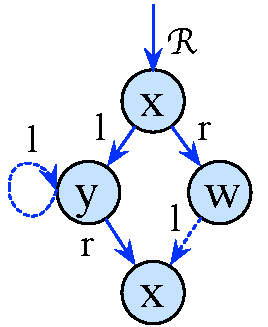
\includegraphics[scale=0.3]{Sections/FurtherExamples/Images/graph.pdf}
    \caption{}
    \label{subfig:graph}
    \end{subfigure}
    &
    \begin{subfigure}[b]	{0.2\columnwidth}		
      \centering	
      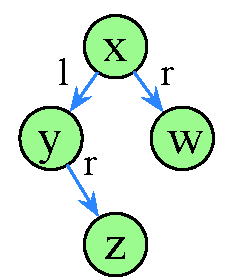
\includegraphics[scale=0.3]{Sections/FurtherExamples/Images/tree.pdf}
    \caption{}
    \label{subfig:tree}
    \end{subfigure}
    &
    \begin{subfigure}[b]{0.3\columnwidth}
      \centering	
      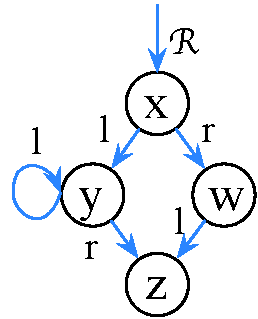
\includegraphics[scale=0.3]{Sections/FurtherExamples/Images/graphWithRootEdge.pdf}
    \caption{}
    \label{subfig:graphWithRootEdge}
    \end{subfigure}
    \end{tabular}
\hrule
\caption{A directed connected binary graph (\subref{subfig:graph}), a possible spanning tree (\subref{subfig:tree}), and the same graph with the logical edge $\rootEdge$ (\subref{subfig:graphWithRootEdge}).}
\label{fig:graphAndTree}
\end{figure}
%Let $\gamma = (V, E)$ denote a connected directed binary graph where $V$ is a finite set of vertices and $E: V \rightarrow (V \uplus \{0\}) \times (V \uplus \{0\})$ is a function associating each vertex with at most two successors. Given a graph $\gamma = (V, E)$, a \emph{tree} (acyclic connected directed graph) $\theta$ is a spanning tree of $\gamma$ if it includes all vertices of $\gamma$ and every edge in $\theta$ is also an edge in $\gamma$. In other words, $\theta = (V, E')$ where $E' \subseteq E$ and $E'$ is minimal. Given a graph $\gamma = (V, E)$, we write $x \in \gamma$ for $x \in V \uplus \{0\}$.

In order to reason about graphs, we define an inductive predicate $\graph{x}{S}$ as given in \fig\ref{fig:globalCST} to describe a graph rooted at address $x$ with the finite set of vertices (addresses) $S$. It represents a spatial (in heap) graph shared amongst the threads spanning it where each node can be marked (visited) via any of its incoming edges from its predecessors. For instance, in the graph of \fig\ref{subfig:graph}, the $z$ node can be visited via the right edge of node $y$ ($y.r$) as well as the left edge of node $w$ ($w.l$). As such, in our reasoning we have \emph{marking} capabilities of the form $\markT{n}{e}$ where $n$ denotes the vertex (address) and $e$ the edge via which vertex $n$ is visited. For instance, the capabilities associated with marking of vertex $z$ in \fig\ref{subfig:graph} are $\markT{z}{y.r}$ and $\markT{z}{w.l}$. Recall from \S\ref{sec:logic} that the parameterisation of our actions are merely a notational convenience and can be substituted for their full definitions. Given a graph  at root address $x$, in order to account for the ability to mark the root vertex $x$, we introduce a logical (virtual) root edge $\rootEdge$ into $x$ as depicted in \fig\ref{subfig:graphWithRootEdge} together with its associated marking capability $\markT{x}{\rootEdge}$. The shared state contains node $x$ which can be either unmarked ($\unmarked{x}{l}{r}$) or marked ($\marked{x}$); as well as the left and right subgraphs captured recursively by the $\G{l}{S}$ and $\G{r}{S}$ predicates. Note that the two subgraphs and vertex $x$ are combined by the overlapping conjunction $\sepish$ since the graph can be cyclic and each node may be reachable via more than one path. 

Each vertex is represented as three consecutive cells in the heap tracking the mark value ($0$ or $1$) and the addresses of the left ($l$) and right ($r$) subgraphs. For brevity, we write $\cell{x}{m, l, r}$ for $\cell{x}{m} * \cell{x+1}{l} * \cell{x+2}{r}$. Moreover, in order to increase readability we write $x.m$, $x.l$ and $x.r$ for $x$, $x+1$ and $x+2$, respectively. When vertex $x$ is in the unmarked state, the mark value corresponds to $0$ ($\cell{x.m}{0}$) and the left and right pointers ($\cell{x.l}{l} * \cell{x.r}{r}$) as well as the capability to mark them ($\markT{l}{x.l} * \markT{r}{x.r}$ reside in the shared state. In the marked state the mark value is $1$ ($\cell{x.m}{1}$) and the resources associated with the left and right subgraphs (pointers and capabilities) have been claimed by the marking thread. 

The interference associated with the graph is described as the union of interferences pertaining to the vertices of the graph ($S$). For each vertex $n \in S$, the only permitted action is that of marking $n$ which can be carried out by any of the marking capabilities associated with node $n$ ($\markT{n}{-}$). Note that the anonymous quantification $-$ is yet another notational shorthand and can be substituted for the following more verbose definition.
%%
%\[
%I(n) \eqdef \bigcup\limits_{p \in S} \left( \bigcup\limits_{e \in \{p.l, p.r, \rootEdge\}} \markT{n}{e} : \exsts{l, r} \unmarked{n}{l}{r} \swap \marked{n} \right)
%\]
%%
%
\[
I(n) \eqdef \bigcup\limits_{e \in \textsf{Loc}} \markT{n}{e} : \exsts{l, r} \unmarked{n}{l}{r} \swap \marked{n} 
\]
%
%
\begin{figure}
%
\hrule
\[
\begin{array}{r @{\hspace*{2pt}} l}
	\graph{x}{S} \eqdef & \markT{x}{\rootEdge} * \shared{\G{x}{S}}{\bigcup\limits_{n \in S}I(n)}\\
%	
	\G{x}{S} \eqdef & (x = \nil \land \emp) \lor x \in S \land \exsts{l, r}\\
	& \left( \unmarked{x}{l}{r} \lor \marked{x}\right) \sepish \G{l}{S} \sepish \G{r}{S}\\
%
	\unmarked{x}{l}{r} \eqdef & \cell{x}{0, l, r} * \markT{l}{x.l} * \markT{r}{x.r}\\
%	
	\marked{x} \eqdef & \cell{x}{1}\\
%
	I(n) \eqdef & \left\{ \markT{n}{-}: \exsts{l, r} \unmarked{n}{l}{r} \swap \marked{n}\right\}\\
%
%	\tree{x}{S} \eqdef & \markT{x}{\rootEdge} * \shared{\G{x}{S}}{\bigcup\limits_{n \in S}I(n)}\\
\end{array}
\]
%
\hrule
\caption{Global specification of the graph predicate.}
\label{fig:globalCST}
\end{figure}
%
%
\fig\ref{fig:conSpanningTree} shows an in place concurrent algorithm for calculating a spanning tree of a graph. It proceeds by recursively marking the vertices to keep track of those already visited; the return value b records the outcome of marking with b=$true$ when the top node $x$ is unmarked (not visited yet) and b=$false$ otherwise. Assuming that the root vertex $x$ is unmarked initially, the algorithm continues by first marking $x$ and subsequently spanning the left and right subgraphs concurrently. When the top node of the left subgraph is already marked (!b1), the edge from $x$ into it is replaced by a null pointer. This corresponds to the case where the node has already been visited by another thread and is thus reachable from the root; \emph{mutatis mutandis} for the right subgraph.
%
\begin{figure}
%
\hrule
\[
\begin{array}{r @{\hspace*{2pt}} l}
	\g{x}{S} \eqdef & (x = \nil \land \emp) \lor x \in S \land \exsts{l, r}\\
	& \shared{\unmarked{x}{l}{r} \lor \marked{x}}{I(x)} * \g{l}{S} * \g{r}{S}\\
	
	\tr{x}{S} \eqdef & (x = \nil \land \emp) \lor \\
	& x \in S \land \exsts{l, r}\exsts{l' \in \{l, \nil\}} \exsts{r' \in \{r, \nil\}}\\
	&  \shared{\marked{x}}{I(x)} * \markT{l}{x.l} * \cell{x.l}{l'} * \tr{l'}{S} * \\
	&  \markT{r}{x.r} * \cell{x.r}{r'} *\tr{r'}{S}
\end{array}
\]
\hrule
\label{fig:localCST}
\caption{Local specification of the graph predicate.}
\end{figure}
%
The $\graph{x}{S}$ predicate defined in \fig\ref{fig:globalCST} is a \emph{global} account of the graph in that it captures all vertices and the interference associated with them. However, our spanning tree algorithm operates \emph{locally} as it is called upon recursively for each node. That is, for each $\texttt{span}(n)$ call (where $n \in S$), the footprint of the call is limited to node $n$. Moreover, in order to reason about the concurrent recursive calls $\texttt{span(x.l) || span(x.r)}$, we need to \emph{split} the state into two $*$-composed states prior to the calls, pass each constituent state onto the relevant thread and combine the resulting states by $*$ composition through an application of the \textsc{Par} rule. We thus provide a \emph{local} specification of the graph, $\g{x}{S}$ as defined in \fig\ref{fig:localCST} such that for all $S in \pset{\textsf{Loc}}$ and $n, e \in S$  \\

\todo explain the $\g{x}{S}$ and $\tr{x}{S}$ predicates. 
%
\[
	\left\{
	\begin{array}{@{} l @{}}
		\markT{n}{p} * \\
		\g{n}{S}
	\end{array}
	\right\}  
%	
	b\texttt{:= span(}n\texttt{)} 
%
	\left\{
	\begin{array}{@{} l @{}}
		\markT{n}{p} * 
		\left(
		\begin{array}{@{} l @{}}
			b \land \tr{n}{S} \lor\\
			\neg b \land \tr{\nil}{S}
		\end{array}
		\right)
	\end{array}
	\right\}
\]
%


We now demonstrate how to obtain the local specification $\g{x}{S}$ from the global specification of \fig\ref{fig:globalCST}. 
When expanding the definition of $\G{x}{S}$, there are two cases to consider depending on whether or not $x = \nil$. In what follows we only consider the case where $x \not= \nil$ since the derivation in the case of $x = \nil$ is trivial.
%
\[
\begin{array}{@{} c @{} l @{}}
	&\shared{\G{x}{S}}{\bigcup\limits_{n \in S} I(n)}  \\
	
	\stackrel{(\textsf{G}\ \defin)}{\implies} & \shared{\exsts{l, r} (\unmarked{x}{l}{r} \lor \marked{x}) \sepish \G{l}{S} \sepish \G{r}{S}}{\bigcup\limits_{n \in S} I(n)} \\
	
	\implies &   \exsts{l, r}  \shared{(\unmarked{x}{l}{r} \lor \marked{x}) \sepish \G{l}{S} \sepish \G{r}{S}}{\bigcup\limits_{n \in S} I(n)} \\
	
	\stackrel{(\textsc{Copy})}{\implies} &
	\exsts{l, r}  
	\shared{(\unmarked{x}{l}{r} \lor \marked{x})  \sepish \G{l}{S} \sepish \G{r}{S}}{\bigcup\limits_{n \in S} I(n)} \\
	& * \shared{(\unmarked{x}{l}{r} \lor \marked{x}) \sepish \G{l}{S} \sepish \G{r}{S}}{\bigcup\limits_{n \in S} I(n)} \\
	& * \shared{(\unmarked{x}{l}{r} \lor \marked{x})  \sepish \G{l}{S} \sepish \G{r}{S}}{\bigcup\limits_{n \in S} I(n)} \\
	
	
	\stackrel{(\textsc{Forget})}{\implies} &
	\exsts{l, r}  
	\shared{\unmarked{x}{l}{r} \lor \marked{x}  }{\bigcup\limits_{n \in S} I(n)} \\
	& * \shared{\G{l}{S}}{\bigcup\limits_{n \in S} I(n)} * \shared{\G{r}{S}}{\bigcup\limits_{n \in S} I(n)} \\
	
	
	
	\stackrel{(?)}{\semimplies} &
	\exsts{l, r}  
	\shared{\unmarked{x}{l}{r} \lor \marked{x}}{\bigcup\limits_{n \in S} I(n)} * \g{l}{S} * \g{r}{S}\\
	
	
	\stackrel{(\textsc{Shift})}{\semimplies} &
	\exsts{l, r}  
	\shared{\unmarked{x}{l}{r} \lor \marked{x} }{I(x)} * \g{l}{S} * \g{r}{S}\\
	
	
	\iffdef & \g{x}{S}
	
\end{array}
\]
%
%
\begin{figure}
\hrule
\begin{lstlisting}
 //$\comment\{\graph{x}{S}\}$
 //$\comment\{\markT{x}{\rootEdge} * \shared{\G{x}{S}}{\bigcup\limits_{n \in S} I(n)}\}$
 //$\comment\{\markT{x}{\rootEdge} * \g{x}{S}\}$
 b:= span(x) {
   //$\comment\{\markT{x}{\rootEdge} * \shared{\exsts{l, r} \unmarked{x}{l}{r} * \g{l}{S} * \g{r}{S}  \lor \marked{x}}{I(x)} \}$
   res:= <CAS(x.m, 0, 1)>;
   //$\comment\left\{\begin{array}{l}\markT{x}{\rootEdge} * \shared{\marked{x}}{I(x)} *\\ (\neg\texttt{res}\land\emp) \lor\\  \left(\begin{array}{l}\texttt{res}\land\exsts{l, r} \cell{x.l}{l} * \cell{x}{r} *\\ \markT{l}{x.l} * \g{l}{S} * \markT{r}{x.r} * \g{r}{S} \end{array}\right)\end{array}\right\}$
   if (res) then { 
   //$\comment\left\{\begin{array}{l} \texttt{res} \land \exsts{l, r} \markT{x}{\rootEdge} * \shared{\marked{x}}{I(x)} * \cell{x.l}{l} * \cell{x}{r} *\\\markT{l}{x.l} * \g{l}{S} * \markT{r}{x.r} * \g{r}{S} \end{array}\right\}$
     //$\comment\left\{\markT{l}{x.l} * \g{l}{S} * \markT{r}{x.r} * \g{r}{S}  \right\}$   
     b1:= span(x.l) || b2:= span(x.r)
     //$\comment\left\{\begin{array}{l}\markT{l}{x.l} * \left( (\texttt{b1} \land \tr{l}{S}) \lor (\neg\texttt{b1} \land \tr{\nil}{S})\right) *\\ \markT{r}{x.r} * \left( (\texttt{b2} \land \tr{r}{S}) \lor (\neg\texttt{b2} \land \tr{\nil}{S})\right)  \end{array}\right\}$   
   //$\comment\left\{\begin{array}{l}  \texttt{res} \land \exsts{l, r} \markT{x}{\rootEdge} * \shared{\marked{x}}{I(x)} * \cell{x.l}{l} * \cell{x}{r} *\\ \markT{l}{x.l} * \left( (\texttt{b1} \land \tr{l}{S}) \lor (\neg\texttt{b1} \land \tr{\nil}{S})\right) *\\ \markT{r}{x.r} * \left( (\texttt{b2} \land \tr{r}{S}) \lor (\neg\texttt{b2} \land \tr{\nil}{S})\right)   \end{array}\right\}$  
     if (!b1) then 
       x.l:= null
     if (!b2) then 
       x.r:= null
   //$\comment\left\{\begin{array}{l}  \texttt{res} \land \exsts{l, r} \markT{x}{\rootEdge} * \shared{\marked{x}}{I(x)} * \\ \exsts{l' \in \{l, \nil\}} \markT{l}{x.l} * \cell{x.l}{l'} * \tr{l'}{S} *\\ \exsts{r' \in \{r, \nil\}} \markT{r}{x.r} * \cell{x}{r'} * \tr{r'}{S} \end{array}\right\}$      
   //$\comment\{\texttt{res} \land \markT{x}{\rootEdge} *  \tr{x}{S}\}$      
   }		
   //$\comment\{(\texttt{res} \land \markT{x}{\rootEdge} * \tr{x}{S}) \lor (\neg \texttt{res} \land \markT{x}{\rootEdge} * \shared{\marked{x}}{I(x)}) \}$   
   //$\comment\{\markT{x}{\rootEdge} *  (\texttt{res} \land \tr{x}{S}) \lor (\neg \texttt{res} \land \tr{\nil}{S}) \}$      
   return res
 }
 //$\comment\{\markT{x}{\rootEdge} *  (\texttt{b} \land \tr{x}{S}) \lor (\neg \texttt{b} \land \tr{\nil}{S}) \}$      
\end{lstlisting}
\hrule\vspace*{5pt}
\caption{Concurrent Spanning Tree Implementation}
\label{fig:conSpanningTree}
\end{figure}
%

\todo Briefly touch the proof of \fig\ref{fig:conSpanningTree}.

\subsection{Set Module}
We now look at the specification of a concurrent set module implemented as a singly-linked list as as described in \cite{cap-ecoop10}. A typical set module provides three functionalities: \command{contains(h,v)}, \command{add(h,v)} and \command{remove(h,v)} specified as follows. The $\inSet{\var{h}}{\var{v}} $ predicate asserts that the set at \var{h} contains value \var{v}. Dually, $\outSet{\var{h}}{\var{v}}$ asserts that the set does not contain \var{v}. As the name suggests, the \command{contains} function checks whether value \var{v} is contained in the set; the \command{add(h,v)} and \command{remove(h,v)} functions add/remove value \var{v} to/from the list, respectively. 
%
\[
\begin{array}{@{} r @{\hspace*{3pt}} c @{\hspace*{3pt}} l @{}}
	\left\{ \inSet{\var{h}}{\var{v}} \right\} & \command{contains(h,v)} & \left\{ \inSet{\var{h}}{\var{v}} * \var{ret} = 1 \right\} \\
	
	\left\{ \outSet{\var{h}}{\var{v}} \right\} & \command{contains(h,v)} & \left\{ \outSet{\var{h}}{\var{v}} * \var{ret} = 0 \right\} \\
	
	\left\{ \inSet{\var{h}}{\var{v}} \lor \outSet{\var{h}}{\var{v}}  \right\} & \command{add(h,v)} & \left\{ \inSet{\var{h}}{\var{v}} \right\}\\ 
	
	\left\{ \inSet{\var{h}}{\var{v}} \lor \outSet{\var{h}}{\var{v}}  \right\} & \command{remove(h,v)} & \left\{ \outSet{\var{h}}{\var{v}} \right\} 
\end{array}
\]
%
%\azaleacomment{ We don't have enough space to cover this here, it will have to go into the tech report. We should mention it here though.}
\begin{figure*}
\hrule
\[
\begin{array}{@{} l @{}}
\begin{array}{@{} r @{\hspace*{3pt}} l @{}}
	\inSet{h}{v} \eqdef & \exsts{\pi, L} \sorted{L} \land v \in L \land \lockT{h}[\pi] * \lsg{h}{h}{-\infty:: L ++\{\infty\} }{\nil}\\

	\outSet{h}{v} \eqdef & \exsts{\pi, L} \sorted{L} \land v \not\in L \land \lockT{h}[\pi] * \lsg{h}{h}{-\infty:: L ++ \{\infty\} }{\nil}\\
	
	\sorted{L} \eqdef & (L  = [] \land \emp) \lor( \exsts{v_0} L = [v_0] \land \emp) \lor \exsts{v_0, v_1, L'} L = v_0 :: (v_1 :: L') \land v_0 < v_1 \land \sorted{v_1:: L'}\\

	\lsg{h}{x}{L}{y} \eqdef & (x = y \land L = [] \land \emp) \lor (\exsts{v, z, L'} L = v::L' \land \shared{\node{x}{v}{z}}{I(h, x)} * \lsg{h}{z}{L'}{y}) \\
%		\lsg{h}{x}{v:: L}{y} \eqdef & \exsts{z} \shared{\node{x}{v}{z}}{I(h, x)} * \lsg{h}{z}{L}{y}\\


	\node{a}{v}{b} \eqdef & \unlockedNode{a}{v}{b} \lor \lockedNode{a}{v}{b}\\

		\unlockedNode{a}{v}{b} \eqdef  & \cell{a}{0, v, b} * \unlockT{a} * \nextT{a}{b} * \lockT{b}
	\hspace*{1cm}
	\lockedNode{a}{v}{b} \eqdef  \cell{a}{1, v} * \nextT{a}{b}\\
\end{array}		\\\\
		
		
	I(h, a) \eqdef 
	\left\{
	\begin{array}{@{} r @ {\hspace*{2pt}}l @{} }
%		\text{//Locking}\hspace*{1.4cm}&\\
		\lockT{a}: &\left\{ \exsts{v, b} \unlockedNode{a}{v}{b} \swap \lockedNode{a}{v}{b}\right\}\\
		
%		\text{//Unlocking}\hspace*{1.1cm}&\\
		\unlockT{a}: & \left\{ \exsts{v, b} \lockedNode{a}{v}{b} \swap \unlockedNode{a}{v}{b}\right\}\\ 
		
%		\text{//Deletion of } v \hspace*{0.8cm}&\\
		\unlockT{a} * \valueT{h}{v}: &
		\left\{
		\begin{array}{@{} l @{}}
			\exsts{v_0, b, c} \lockedNode{a}{v_0}{b} * \lockedNode{b}{v}{c} \swap \lockedNode{a}{v_0}{c} * \lockedNode{b}{v}{c}\\
			\exsts{v_0, b, c} \lockedNode{b}{v_0}{c} * \lockedNode{a}{v}{c} \swap \lockedNode{b}{v_0}{c}
			
		\end{array}
		\right\}\\ 

		
%		\text{//Insertion of } v \hspace*{0.7cm}&\\
		\unlockT{a} * \valueT{h}{v}: &
		\left\{
		\begin{array}{@{} l @{}}
			\exsts{v_1, v_2, c, d} v_1 < v < v_2 \land \lockedNode{a}{v_1}{c} * \lockedNode{c}{v_2}{d} 
			 \swap \lockedNode{a}{v_1}{b} * \node{b}{v}{c} *  \lockedNode{c}{v_1}{d}\\
			 
			 \exsts{v_1, v_2, c, d} v_1 < v < v_2 \land \lockedNode{a}{v_1}{c} * \unlockedNode{c}{v_2}{d} 
			\swap \lockedNode{a}{v_1}{b} * \node{b}{v}{c} *  \unlockedNode{c}{v_1}{d}
						
		\end{array}
		\right\}\\ 
		
	\end{array}
	\right\}

\end{array}
\]
\hrule
\caption{Set specification where the definition of .}
\label{fig:setExample}
\end{figure*}

\subsection*{Related Work and Concluding Remarks}

Compositional reasoning about fine-grained concurrent algorithms is
essential for verifying large concurrent systems.  Jones introduced
global rely-guarantee thinking in his PhD
thesis~\cite{rg}, motivating the rely and guarantee relations given in
\S\ref{sec:semantics}. O'Hearn introduced local concurrent separation
reasoning~\cite{csl-tcs}, giving the disjoint concurrency rule
which underpins the reasoning presented here.  Since then, many
researchers 
have looked at more complex and finer-grained algorithms,
building on the combination of global and local  ideas arising from these papers:
examples include RGSep~\cite{viktor-marriage}, Local RG~\cite{lrg},
deny-guarantee~\cite{dg}, and the CAP
family~\cite{cap-ecoop10,icap,tada}, to name but a few. In addition,
the views framework~\cite{views} clarifies much of the basic assumptions associated
with this work: assertions provide disjoint 
\emph{views} of the concrete machine state for each thread, which
other threads cannot invalidate. 


One point of inspiration has come from CAP reasoning. 
CAP uses boxed assertions of the form $\capbox{P}{I}{r}$,
where the assertion $P$ describes a fixed disjoint  part of the global shared
state labelled by fixed region name  $r$, and the interference given by $I$ is also fixed. In contrast,
\colosl uses overlapping  subjective views $\shared{P}{I}$ with no region name, where
assertion $P$ now describes a flexible, overlapping part of the global
shared state, and there is a subtle dynamic relationship between this
$P$ and 
the flexible $I$. Subjective views  lead to simpler proofs, as 
illustrated by the concurrent set example in
\S\ref{sec:examples}. There are many interesting ideas present in the CAP
literature: e.g. abstract states~\cite{carasel}; higher-order
reasoning~\cite{icap}; and abstract atomicity~\cite{tada}. All these
ideas require further investigation. Here, our aim was to simply  introduce 
subjective views as a 
fundamental new way of  underpinning of  such reasoning. 



Our merging of overlapping subjective views relies on the overlapping
conjunction introduced in~\cite{rey-slnotes,js-popl12,ramification}.
In~\cite{ramification}, a sequential spanning tree algorithm is
verified using a this connective. \colosl is naturally able to verify
a concurrent tree spanning algorithm where the overlapping of shared
subgraphs is key.



Finally, probably the work that is nearest in spirit to  \colosl is
Local RG~\cite{lrg}. This work provides {\em some}  flexibility in using
assertions to describe the global shared state,
 albeit only
when the assertions describe disjoint parts of the shared state  and when
the interference is  also disjoint. Moreover, Local
RG assertions are specified globally over the entire shared state
using rely/guarantee reasoning, and
cannot be dynamically shifted, in contrast with
\colosl. Nonetheless, both approaches share a similar goal of enabling
more compositional reasoning about the shared state.

%%  where the
%% reasoning is based on the combination of global rely-guarantee reasoning with
%% local separation logic based on one global shared state. 

%% taken inspiration from them. our set example better. 





%Future work: because we are able to specify shared state and
%interferences locally, there is hope that \colosl can be adapted to
%reason about distributed systems as well, as in our motivating example
%of \S\ref{sec:intuition}.

%\julescomment{This is a brain dump. Doesn't have to make it in the
 % submitted version.}

%One of the new paradigms of \colosl is the ability to manipulate the
%interference relation, via \emph{shifting}. The focus of this paper
%has largely been on manipulations of the spatial components of
%subjective views, and the treatment of shifting has been left at the
%minimum we needed to cover our range of examples. This opens the way
%to more fine-grained reasoning about interferences. For instance, a
%process who never receives a capability could safely over-approximate
%the corresponding interference. Conversely, a process who never gives
%a capability away could safely under-approximate the corresponding
%interference relation. In \colosl, this is not yet allowed, as
%interferences can only be shifted to equivalent ones, the only
%exception being the ability to forget actions that have no visible
%effect on the current subjective state. One could imagine tracking
%which process is allowed to own which capability to be more flexible
%in this instance. (if that can be useful at all?)


% POPL recommends abbrvnat bibliography style.
%% \bibliographystyle{abbrvnat}

\begin{spacing}{0.85}
\bibliographystyle{plain_better}
\bibliography{biblio}
\end{spacing}
% The bibliography should be embedded for final submission.


\end{document}
